
\appendix

\setcounter{table}{0}
\setcounter{figure}{0}
\renewcommand{\thetable}{A.\arabic{table}}
\renewcommand{\thefigure}{A.\arabic{figure}}



\section{Metrics\label{appendix:metrics}}
\paragraph{Localization -- positive micro F$_1$ (pmF$_1$):}
For a datapoint with $N$ predicted masks $\{m_i\}_{i=1}^N$ and $M$ ground-truth masks $\{\hat m_j\}_{j=1}^M$, we compute the IoU matrix
\begin{equation}
\mathrm{IoU}_{ij} = \mathrm{IoU}(m_i, \hat m_j).
\end{equation}
We then compute an optimal bipartite assignment (Hungarian matching) $\sigma$ maximizing total IoU. For an IoU threshold $\tau$, a prediction $i$ is a true positive if it is matched and $\mathrm{IoU}_{i,\sigma(i)} \ge \tau$; otherwise it is a false positive. Unmatched ground-truth masks are false negatives. Let $TP_\tau$, $FP_\tau$, and $FN_\tau$ denote the resulting counts. We compute a micro-F$_1$ at threshold $\tau$ by accumulating these counts across all \emph{positive} datapoints (those with $M>0$),
\begin{equation}
\mathrm{pmF_1}_\tau =
\frac{2\,TP_{\tau,\mathrm{total}}}{2\,TP_{\tau,\mathrm{total}} + FP_{\tau,\mathrm{total}} + FN_{\tau,\mathrm{total}}}.
\end{equation}
Following SAM3, we evaluate at 10 thresholds $\tau \in \{0.50, 0.55, \dots, 0.95\}$ and average:
\begin{equation}
\mathrm{pmF_1} = \frac{1}{10}\sum_{\tau}\mathrm{pmF_1}_{@\tau}.
\end{equation}
We also report the per-threshold values (\eg, $\mathrm{pmF_1}_{@0.50}$ and $\mathrm{pmF_1}_{@0.75}$) when relevant.

\paragraph{Classification -- image-level MCC (IL\_MCC):} We adopt the same image-level presence classification metric as SAM3: we treat each datapoint as a binary decision (object present vs.\ not present) based on whether the model predicts any mask, and summarize the resulting confusion matrix with the Matthews Correlation Coefficient (IL\_MCC). We refer readers to SAM3 for the exact definition and implementation details.

\paragraph{Combined -- classification-gated F$_1$ (cgF$_1$):}
Combining localization and classification:
\begin{equation}
\mathrm{cgF_1} = \mathrm{pmF_1}\cdot IL\_\mathrm{MCC}.
\end{equation}


\paragraph{Macro-F$_1$ (per-sample):}
In addition to micro aggregation, we report a macro variant computed as the mean of per-sample scores. For positive samples, the per-sample score is the mean local F$_1$ across thresholds; for true negatives (no ground truth and no prediction) the per-sample score is set to $1$, while false positives and false negatives receive $0$. This metric highlights per-image stability rather than being dominated by high-mask-count samples.






\section{Architecture Study}
\label{sec:arch}



\begin{figure}[t]
\centering

\begin{minipage}{0.72\linewidth}
\centering
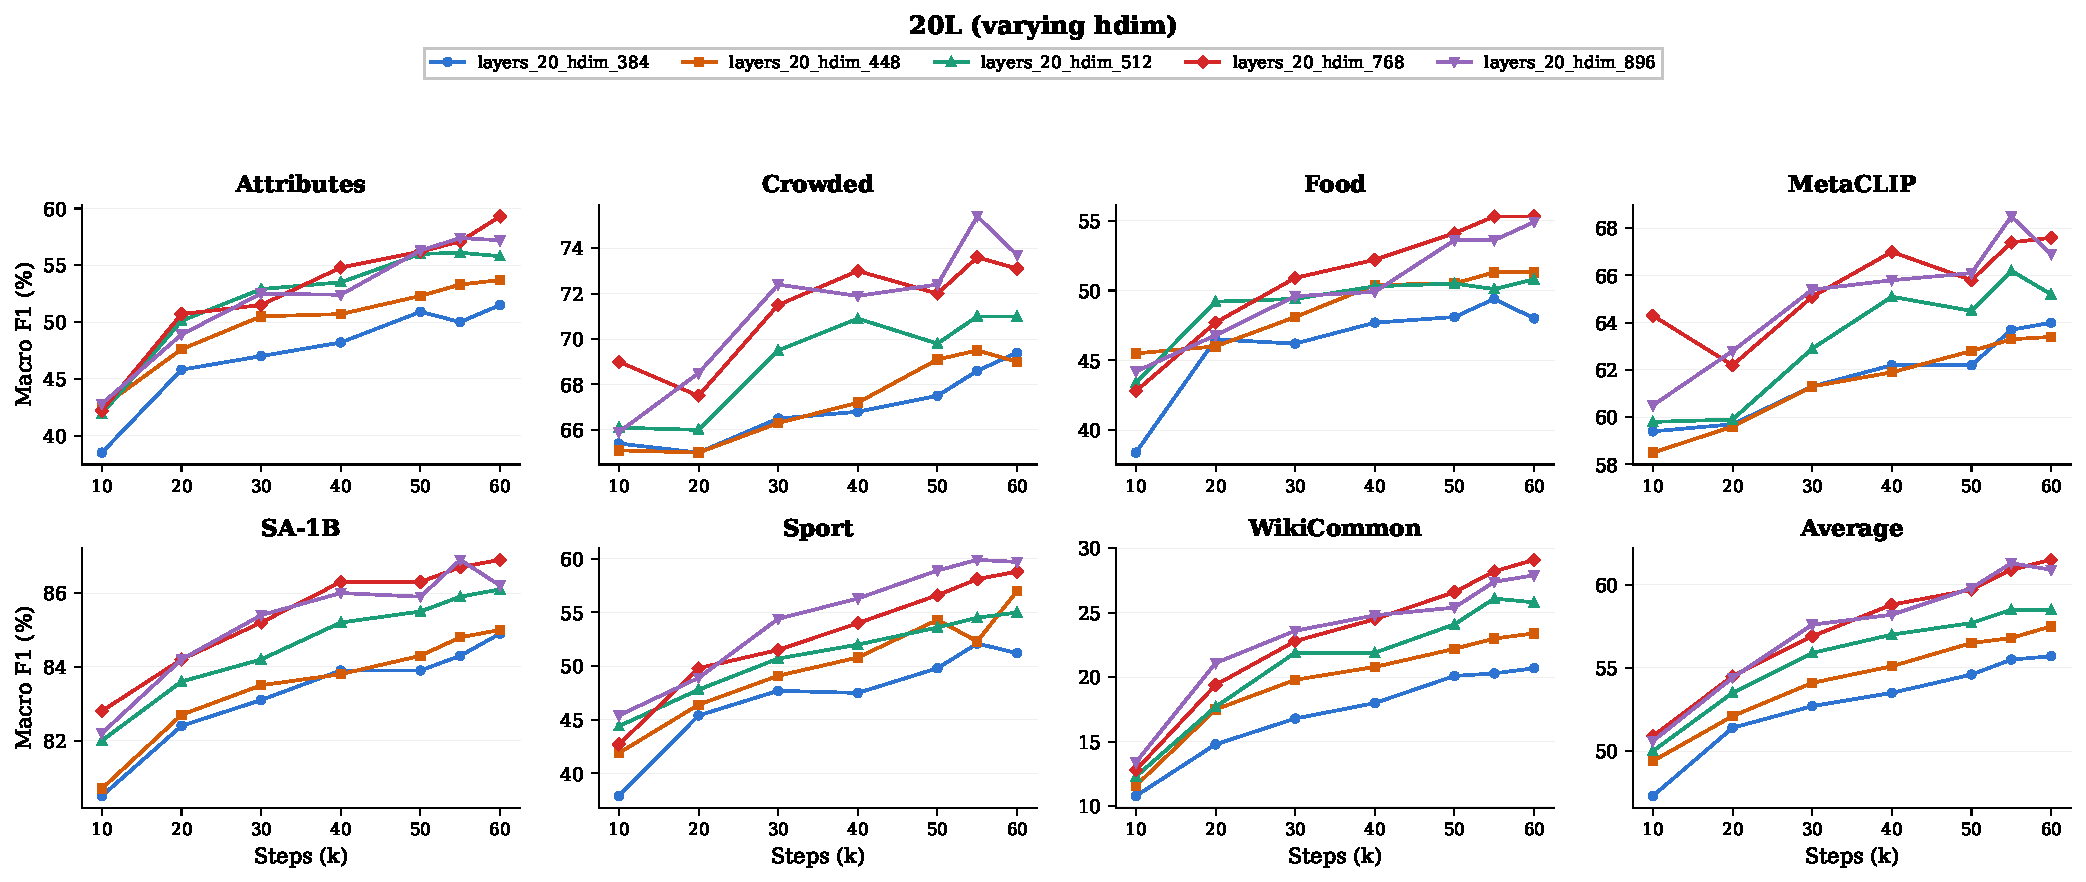
\includegraphics[width=\linewidth, trim=7cm 13.6cm 7cm 0, clip]{figures/sweeps/det_20l_hdim_macro_F1} \\
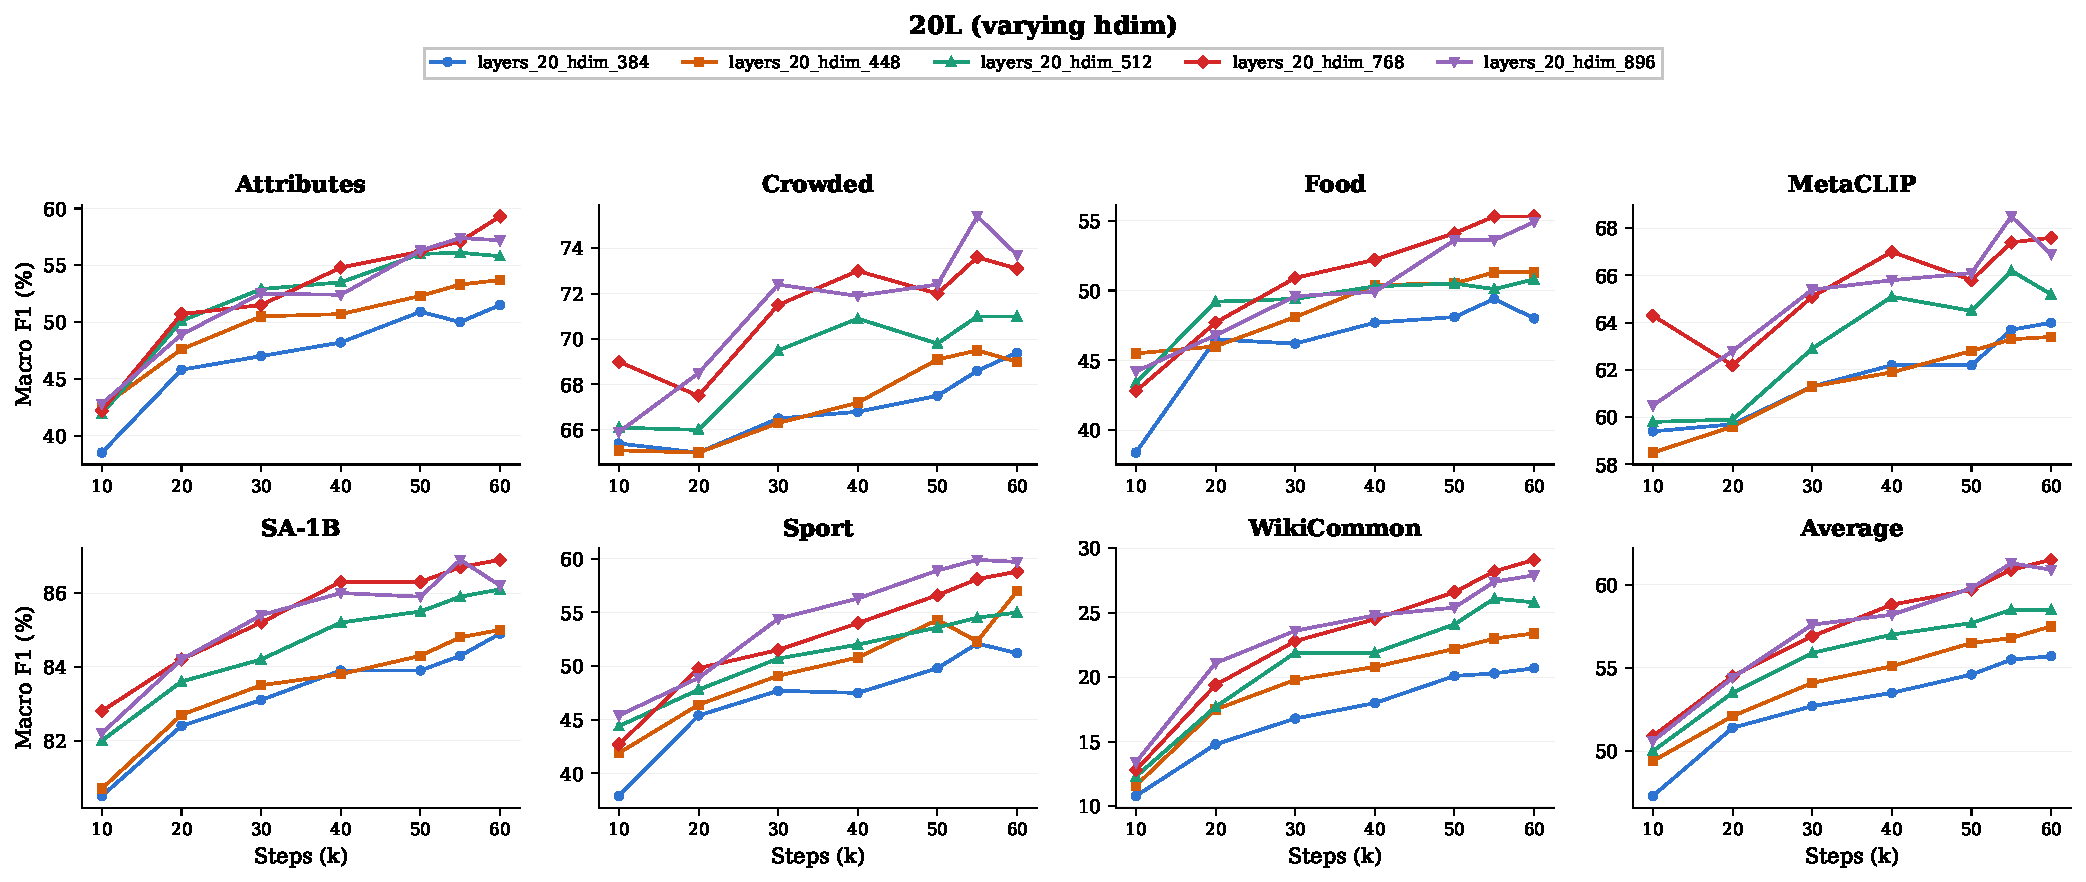
\includegraphics[width=\linewidth, trim=0 0 0 2.5cm, clip]{figures/sweeps/det_20l_hdim_macro_F1}
\end{minipage}
\hfill
\begin{minipage}{0.25\linewidth}
\centering
{\footnotesize
\captionof{table}{Metrics averaged over the seven SaCo splits at 60k steps.\vspace{-0.3cm}\label{tab:appendix_width}}}
\setlength{\tabcolsep}{6pt}
\adjustbox{width=\textwidth}{
\begin{tabular}{cc|cc}
\toprule
$L$ & $d_{\text{model}}$ & MCC & Macro F$_1$ \\
\midrule
20 & 384  & 46.4 & 55.7 \\
20 & 448  & 48.2 & 57.5 \\
20 & 512  & 49.8 & 58.5 \\
20 & 768  & \textbf{53.2} & \textbf{61.5} \\
20 & 896  & 52.4 & 60.9 \\
\bottomrule
\end{tabular}
}
\end{minipage}
\caption{\textbf{Impact of architectural choices:} Width scaling at fixed depth ($L{=}20$). \label{fig:appendix_arch_width}}
\end{figure}

\begin{figure}[t]


\begin{minipage}{0.72\textwidth}
\centering
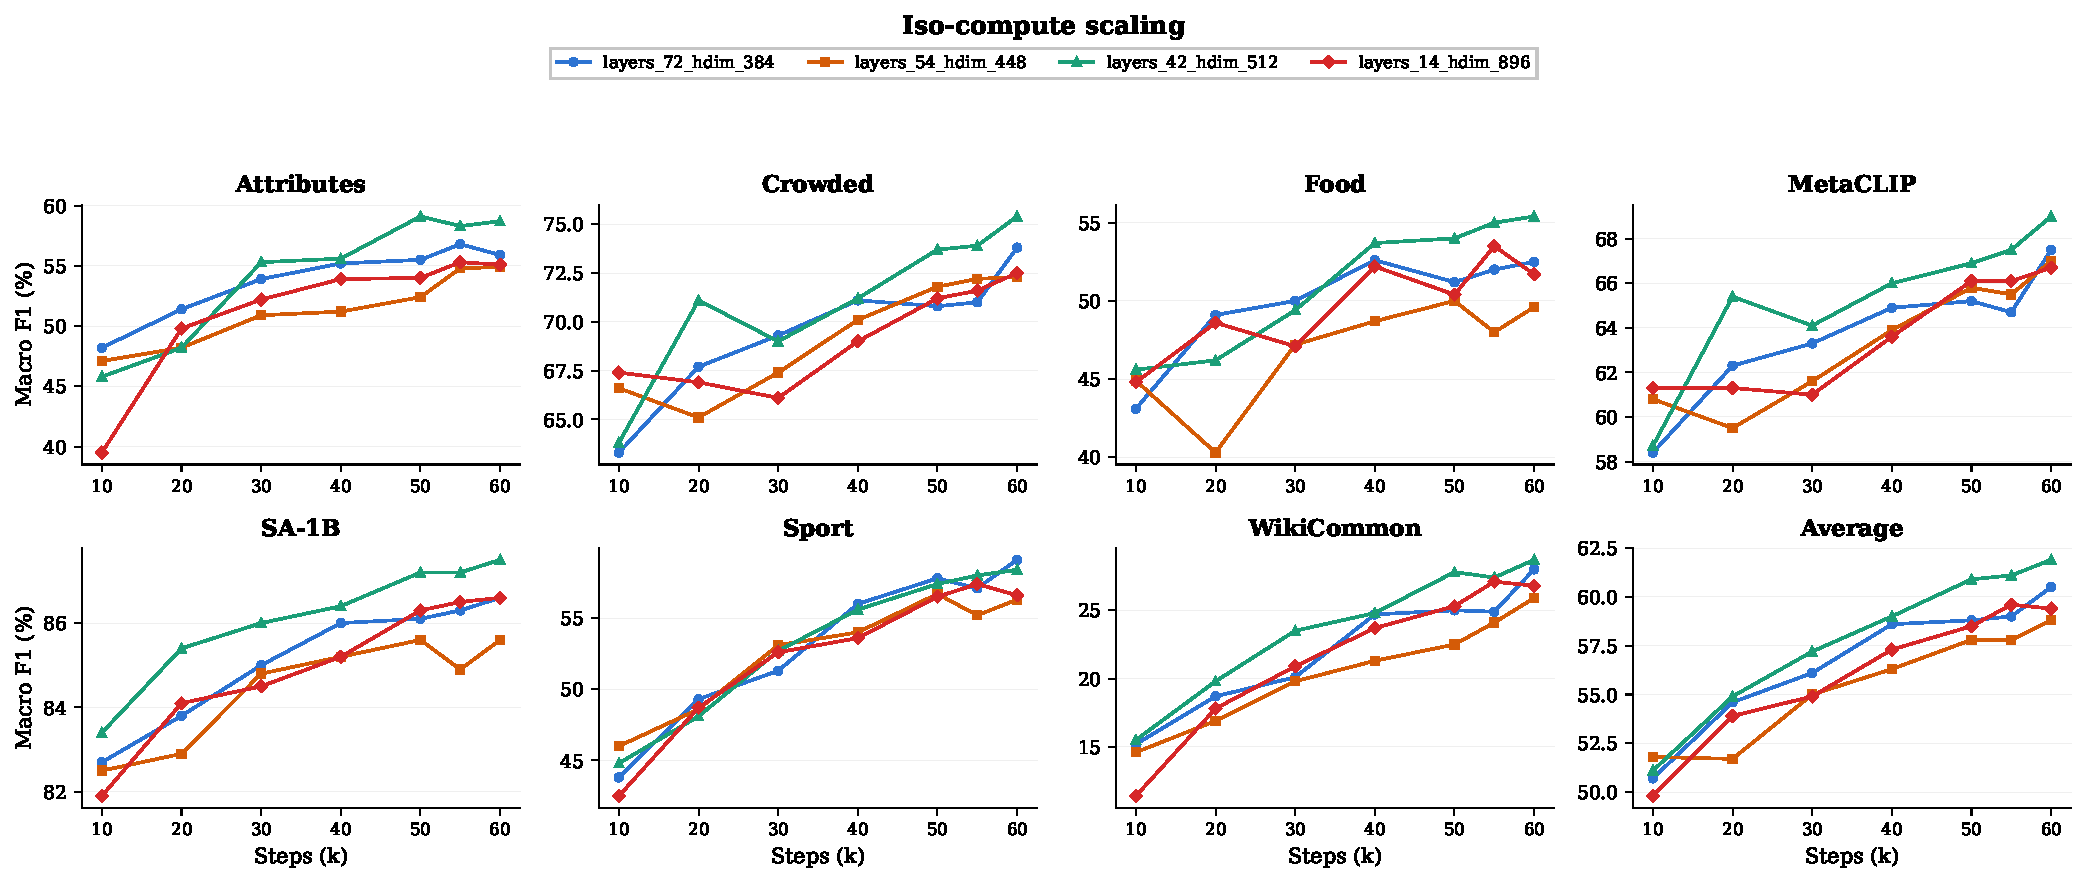
\includegraphics[width=\linewidth, trim=7cm 13.6cm 7cm 0, clip]{figures/sweeps/det_iso_compute_macro_F1.pdf} \\
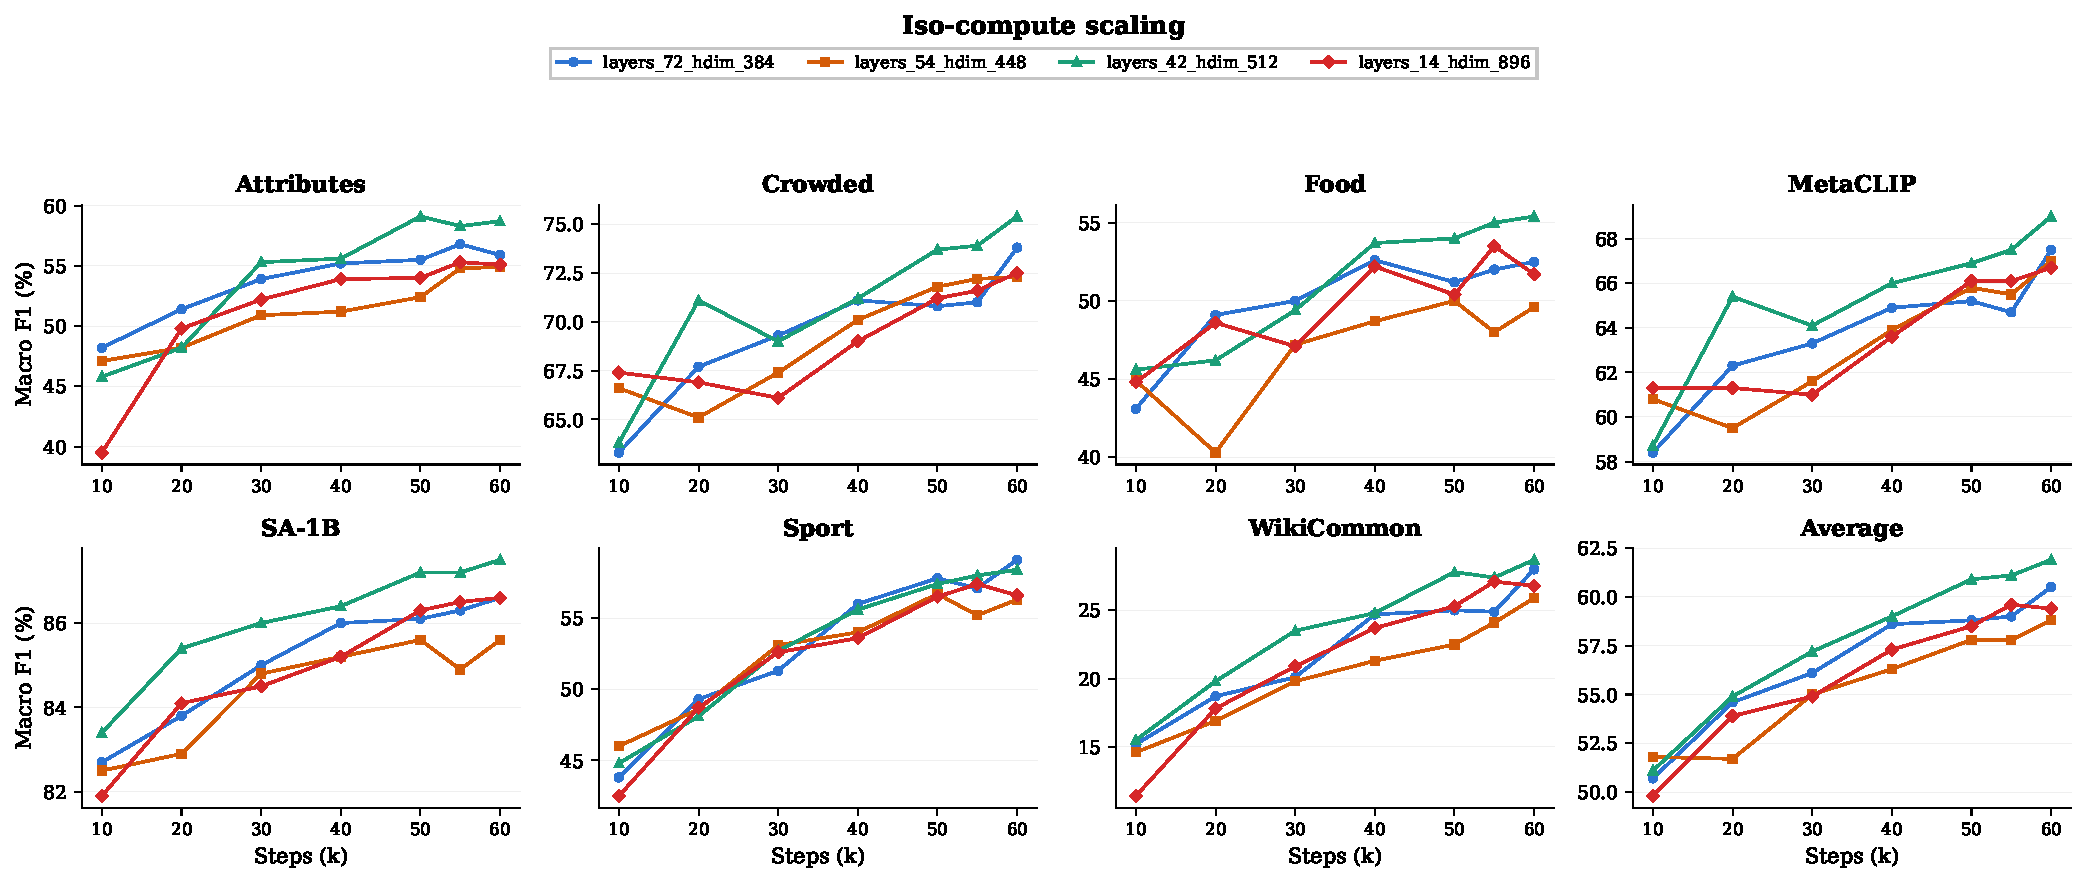
\includegraphics[width=\linewidth, trim=0 0 0 2.5cm, clip]{figures/sweeps/det_iso_compute_macro_F1.pdf}
\end{minipage}
\hfill
\begin{minipage}{0.25\textwidth}
\centering
{\footnotesize
\captionof{table}{Metrics averaged over the seven SaCo splits at 60k steps.\vspace{-0.3cm}\label{tab:appendix_isocompute}}}
\adjustbox{width=\textwidth}{
\begin{tabular}{cc|cc}
\toprule
$L$ & $d_{\text{model}}$ & MCC & Macro F$_1$ \\
\midrule
72 & 384   & 52.4 & 60.5 \\
54 & 448   & 50.0 & 58.8 \\
42 & 512   & \textbf{54.0} & \textbf{61.9} \\
20 & 768   & 53.2 & 61.5 \\
14 & 896   & 50.8 & 59.4 \\
\bottomrule
\end{tabular}
}
\end{minipage}

\caption{\textbf{Impact of architectural choices:} Iso-compute depth--width trade-off.}
\label{fig:appendix_arch_isocompute}

\end{figure}

A central design question for unified dense-prediction architectures is how to
distribute model capacity between depth (number of layers~$L$) and width
(hidden dimension~$d_{\text{model}}$).  Because visual features and
autoregressive task tokens share the same transformer stack, there is a risk
of \emph{modality crowding}: the channel bandwidth may become a bottleneck
when both modalities compete for representational capacity.  We investigate
this through two controlled studies on the SaCo benchmark, evaluating
bounding-box detection at an IoU threshold of~$0.75$ and reporting the average
MCC and Macro~F$_1$ across all seven splits after 60k training steps.

\paragraph{Hyperparameter transfer:}
To ensure that performance differences reflect architectural capacity rather
than optimization artifacts, we adopt the Maximal Update Parameterization
($\mu$P)~\citep{yang2019wide} for learning-rate transfer across widths.  We
first tune the optimal learning rate on a reference configuration
(20L\,/\,$d_{\text{model}}{=}768$) and transfer it to every other width via
\begin{equation}
  \mathrm{lr}_{\text{target}}
  = \mathrm{lr}_{\text{ref}}
    \cdot \sqrt{\frac{d_{\text{target}}}{d_{\text{ref}}}}\,,
  \label{eq:mup}
\end{equation}
so that the effective magnitude of weight updates remains consistent
regardless of hidden dimension.  All other hyperparameters are kept identical
across configurations.

\subsection{Width Scaling at Fixed Depth}
\label{sec:width}



We fix the network depth at $L{=}20$ layers and vary the hidden dimension
across $d_{\text{model}} \in \{384,\, 448,\, 512,\, 768,\, 896\}$.
Results are summarized in Table~\ref{tab:appendix_width} and Figure~\ref{fig:appendix_arch_width}.
Performance improves monotonically from $d_{\text{model}}{=}384$
(MCC\,$=$\,46.4, F$_1$\,$=$\,55.7) to $d_{\text{model}}{=}768$
(MCC\,$=$\,53.2, F$_1$\,$=$\,61.5), a gain of \textbf{+6.8}~MCC and
\textbf{+5.8}~Macro~F$_1$.  Increasing width further to~896 yields a slight
regression (MCC\,$=$\,52.4), indicating that at 20~layers the architecture
saturates around $d_{\text{model}} \approx 768$.  The sharp degradation at
small widths is consistent with a capacity-bottleneck effect: when visual and
language features must share a narrow hidden state, neither modality is
adequately represented.

\subsection{Depth--Width Trade-off at Fixed Compute}
\label{sec:isocompute}

To disentangle width from overall scale, we fix an approximate compute budget
of 300M parameters and sweep the aspect
ratio across five configurations spanning a~$5{\times}$ range in depth.
Results are shown in Table~\ref{tab:appendix_isocompute} and
Figure~\ref{fig:appendix_arch_isocompute}.
The two balanced configurations: 42L\,/\,512 (MCC\,$=$\,54.0,
F$_1$\,$=$\,61.9) and 20L\,/\,768 (MCC\,$=$\,53.2,
F$_1$\,$=$\,61.5) achieve the highest scores and lie within one~MCC point
of each other.  Both substantially outperform the extremes: the
deepest-narrowest variant (72L\,/\,384: MCC\,$=$\,52.4) and the
shallowest-widest variant (14L\,/\,896: MCC\,$=$\,50.8) each trail the best
configuration by 2--4~points.  Notably, the 54L\,/\,448 model
(MCC\,$=$\,50.0) under\-performs 72L\,/\,384 despite having a wider hidden
state, suggesting that this particular depth--width combination falls into an
unfavorable operating regime.

\subsection{Discussion}

Both studies converge on two findings:
\begin{enumerate}[nosep,leftmargin=*]
  \item \textbf{Width is necessary but not sufficient:}
        Study~A shows that widening the hidden dimension from 384 to 768
        yields a +6.8~MCC improvement at fixed depth, confirming that
        sufficient channel capacity is critical for dense prediction in a
        unified stack.  However, gains saturate beyond
        $d_{\text{model}} \approx 768$.

  \item \textbf{Balanced aspect ratios are optimal under iso-compute:}
        Study~B shows that, for a fixed compute budget, moderate
        configurations (42L\,/\,512 and 20L\,/\,768) outperform both
        deep-narrow and shallow-wide extremes by 2--4~MCC.  This indicates
        that representational diversity from depth and channel capacity from
        width are independently necessary and neither alone compensates for a
        deficit in the other.
\end{enumerate}
Taken together, these results suggest that the unified single-stack
architecture does not inherently suffer from modality crowding.  The optimal operating point in our
explored range is 42L\,/\,512, though 20L\,/\,768 offers a competitive
alternative at a shallower depth that may be preferable when inference latency
is a consideration.




\section{Qualitative Analysis}


\subsection{Image Feature Quality}
Here, we assess the quality of the image features output by our model, which employs early fusion of the image and text tokens. Figure~\ref{fig:appendix_pca} shows the PCA maps of the image features at the Falcon Perception output layer (before the AnyUp feature upsampler) and after being upsampled by the upsampler. We observe that our model learns to distinguish between objects in the image to a reasonable extent, as evident in the image features before upsampling (\eg, the \textit{coffee cup, notebook} and \textit{pen} in the fourth row on the left are clearly distinguishable in the image features before upsampling). Furthermore, at the feature upsampler output, the image features are enhanced with high-fidelity and the instances are better visible, indicating that the features output by our model before upsampling encompass sufficient scene information that is required for promptable instance segmentation. These results show the effectiveness of early fusion design in our Falcon Perception.
\begin{figure}[t]
  \centering


\begin{minipage}{0.5\textwidth}
\centering
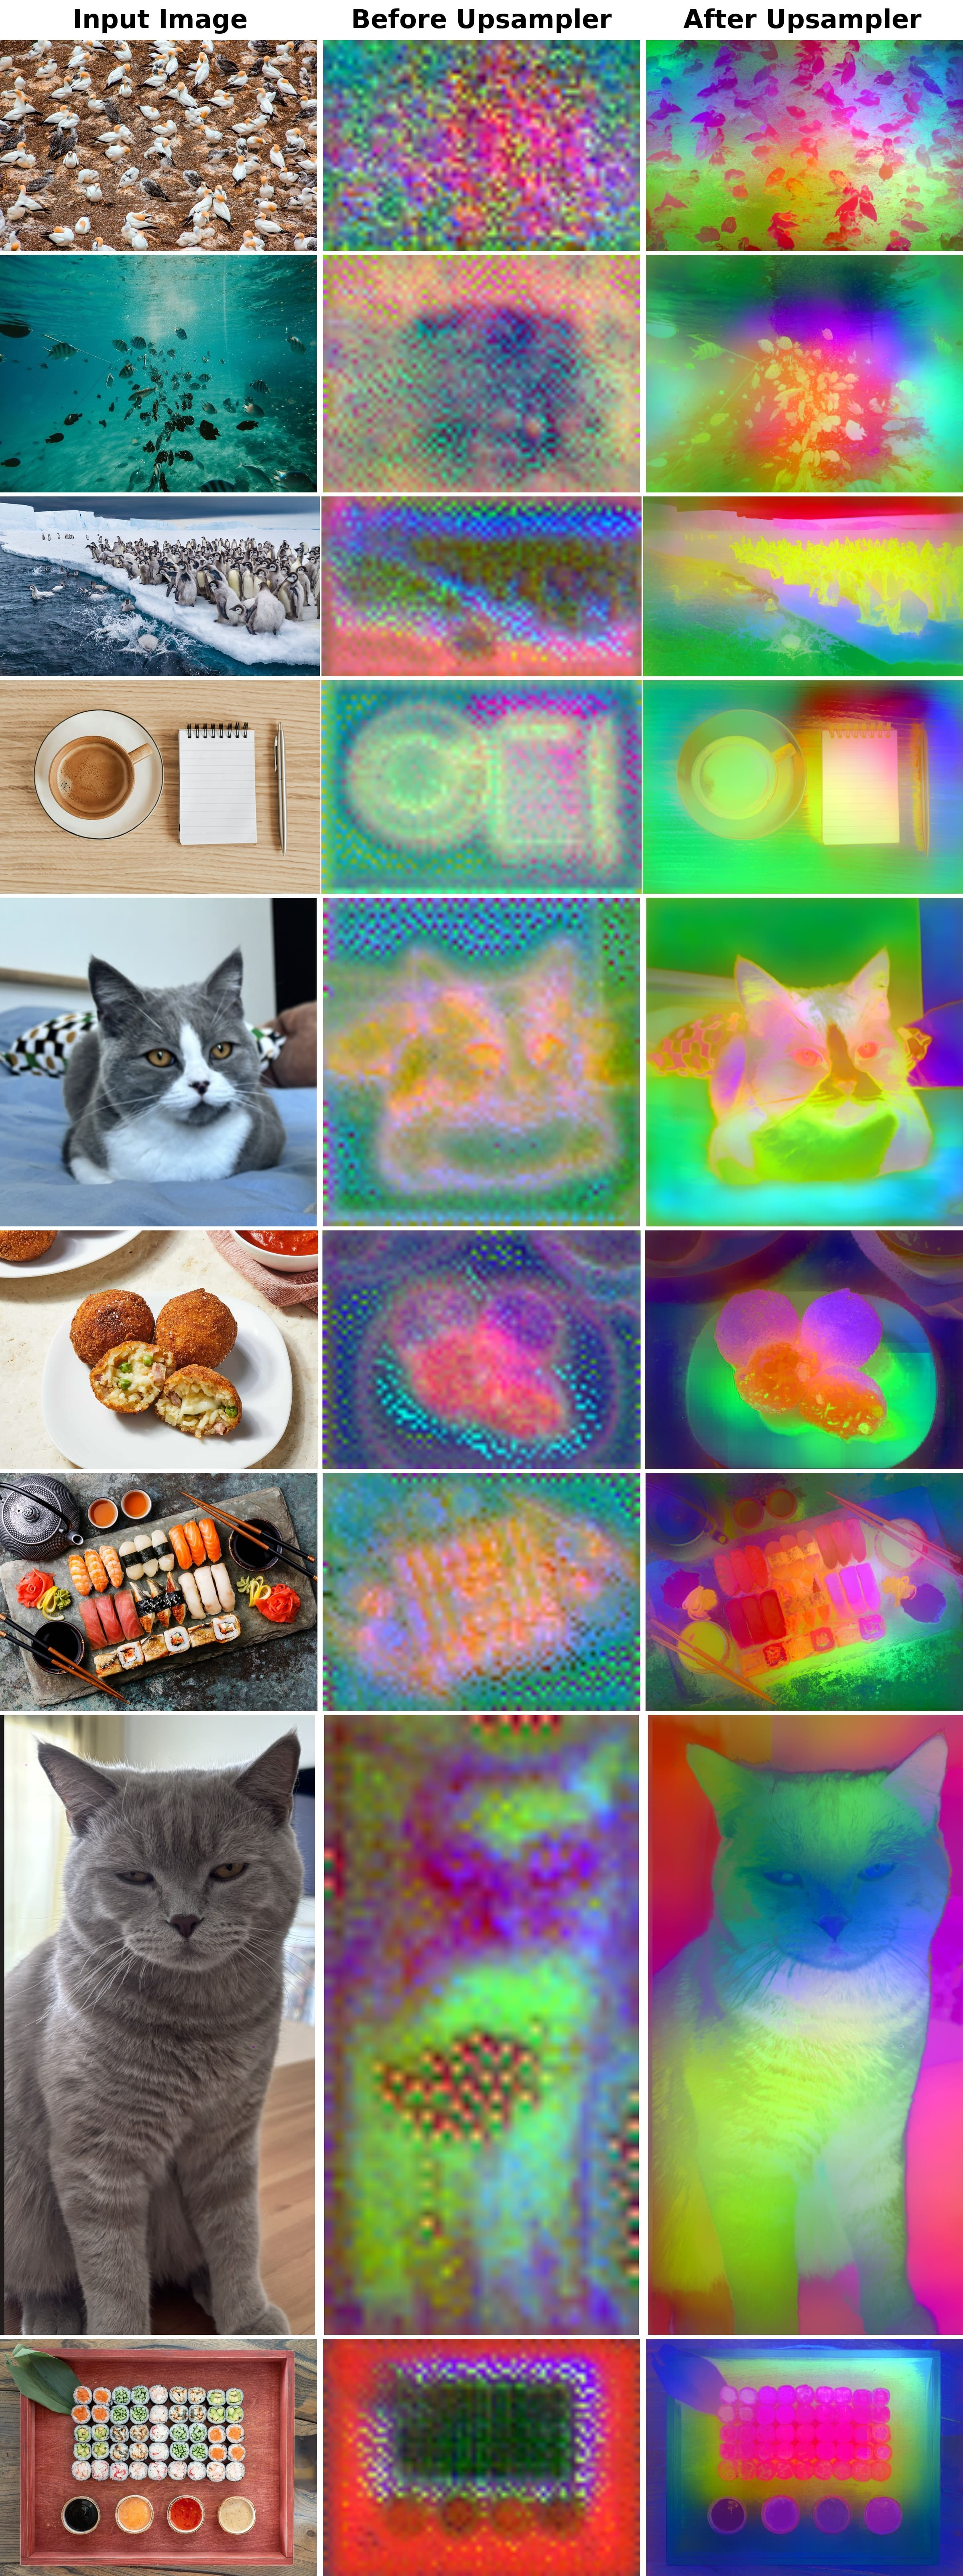
\includegraphics[width=\textwidth, trim=0 120cm 0 0, clip]{figures/pca_comparisons.jpg}
\end{minipage}
\hfill
\begin{minipage}{0.49\textwidth}
\centering
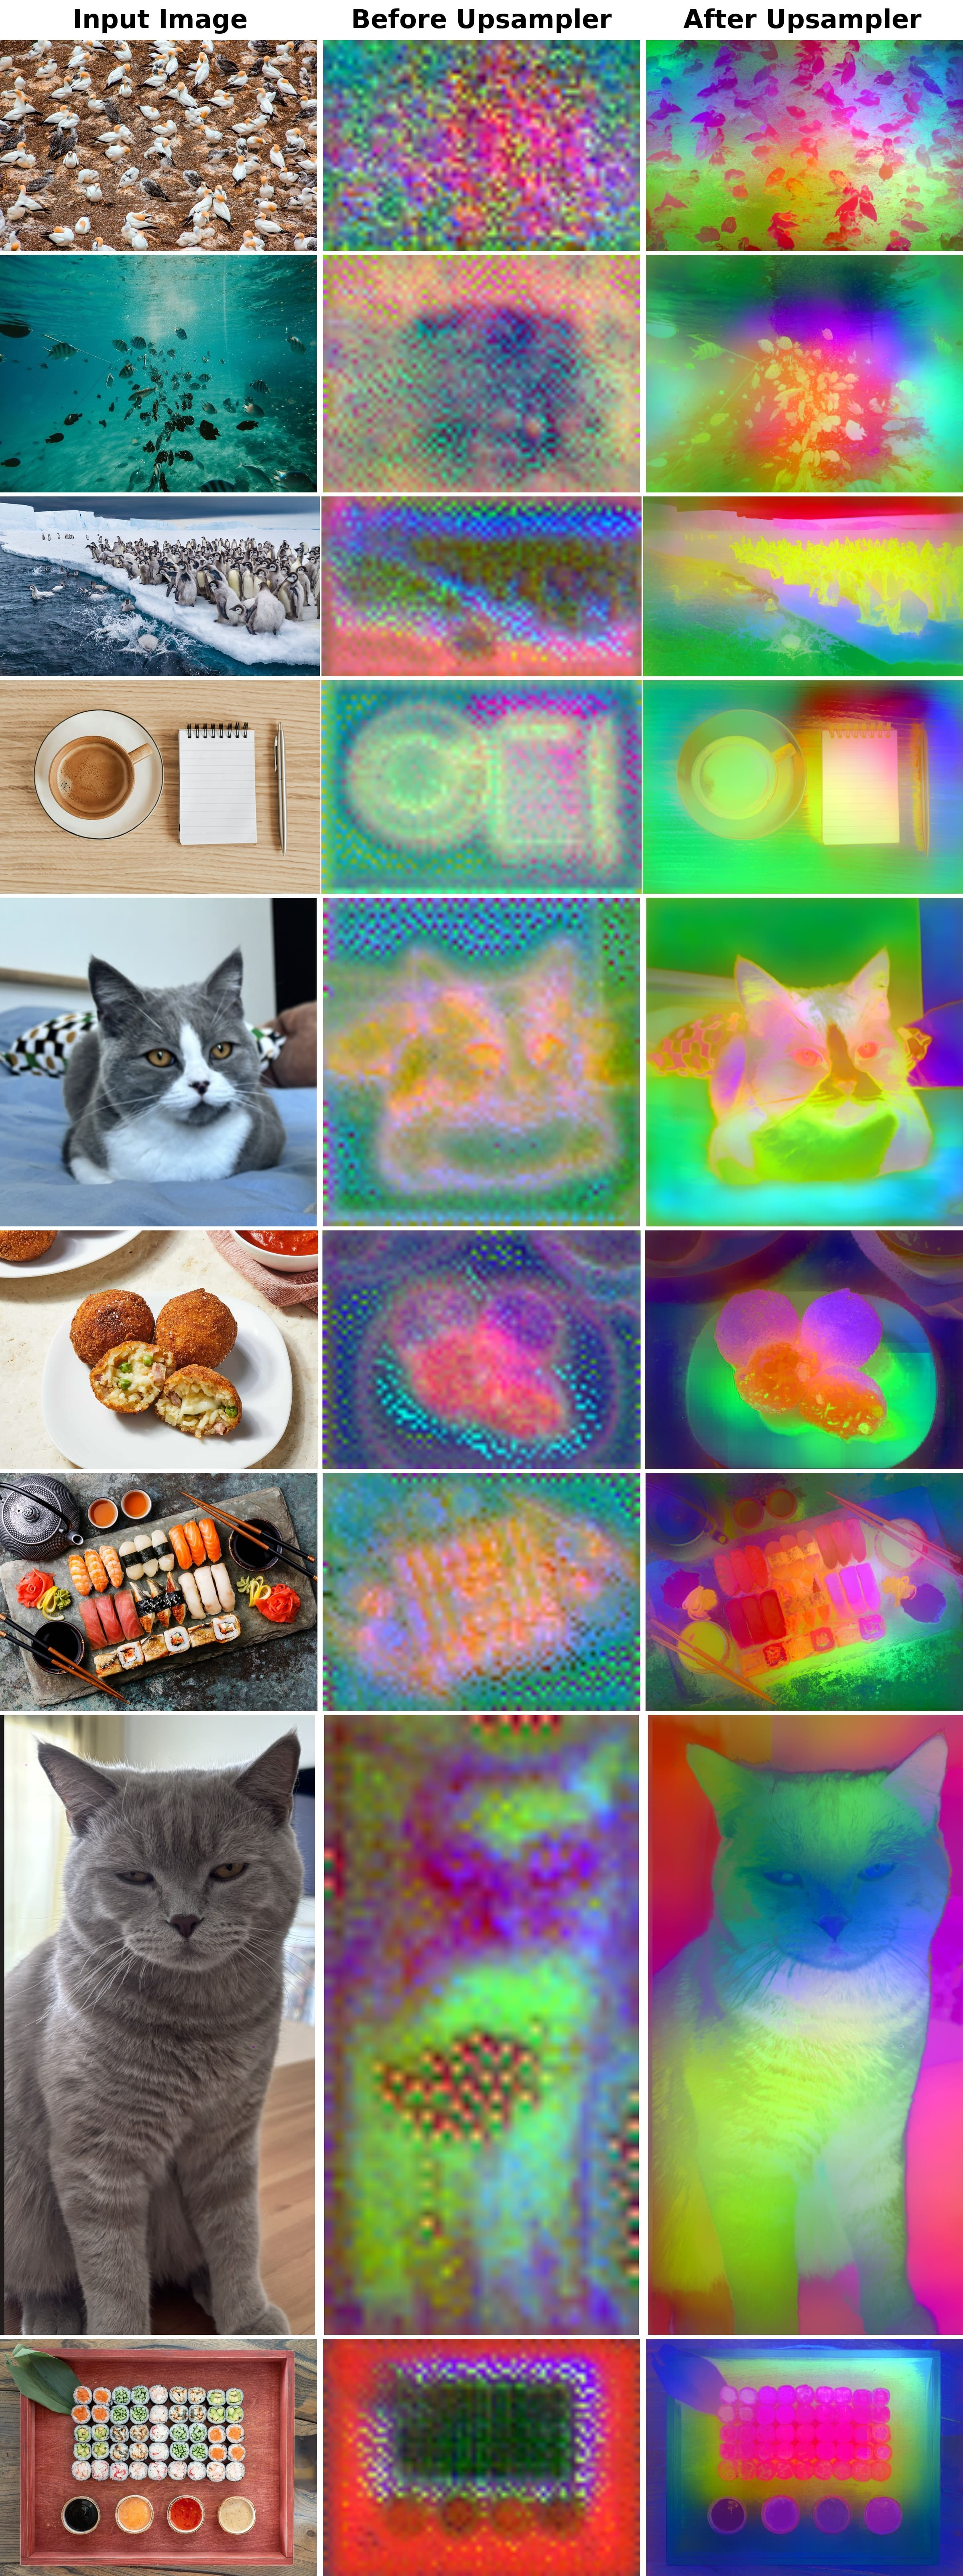
\includegraphics[width=1\textwidth, trim=0 223.5cm 0 0, clip]{figures/pca_comparisons.jpg}\\
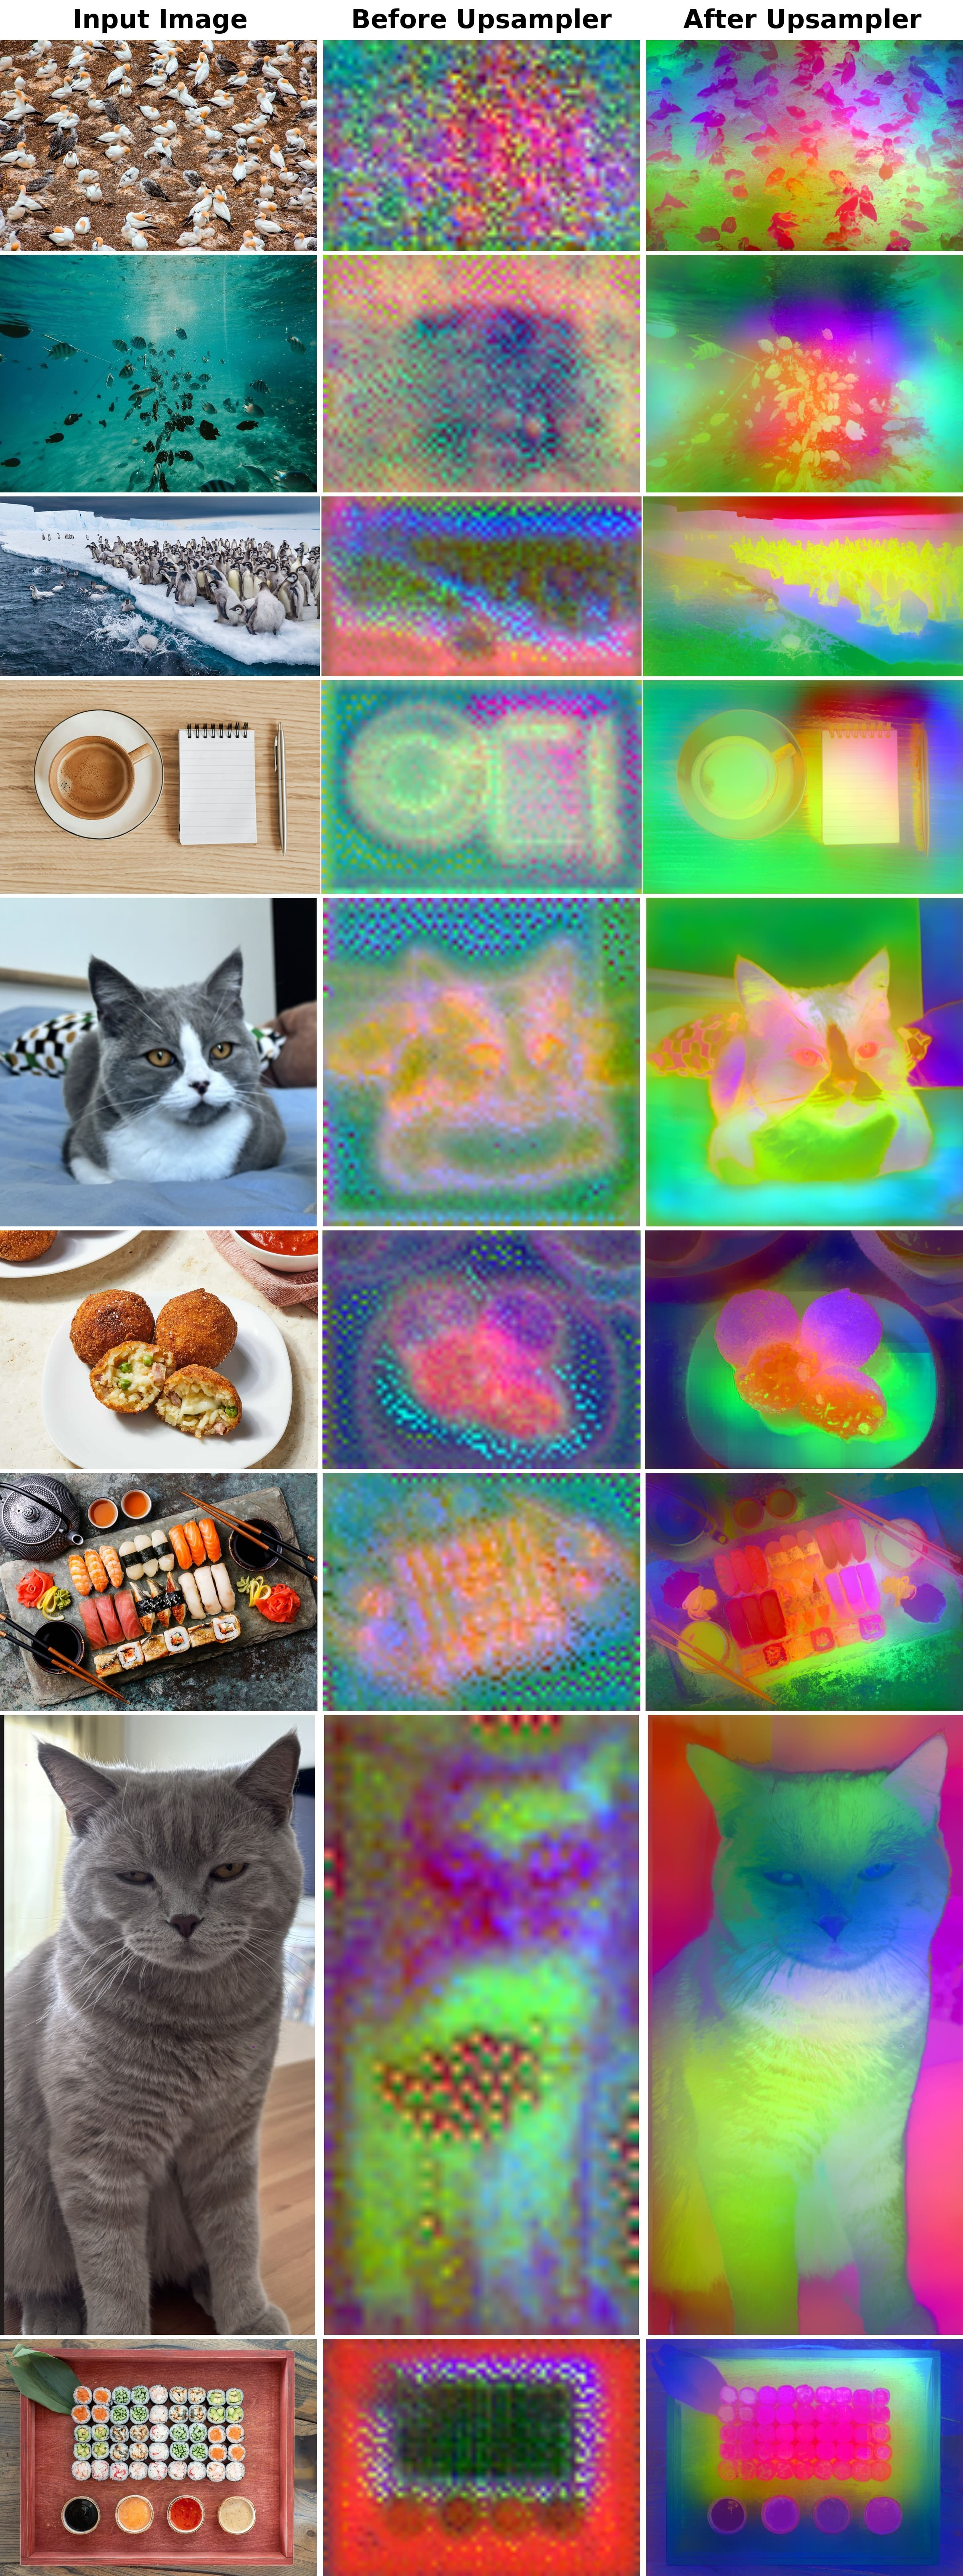
\includegraphics[width=0.95\textwidth, trim=0 0 0 110cm, clip, height=0.392\textheight]{figures/pca_comparisons.jpg}
\end{minipage}
\vspace{-0.1cm}
\caption{\textbf{PCA maps before and after upsampling:} Image features before upsampling already distinguish multiple objects, \eg, the \textit{coffee cup, notebook}, and \textit{pen} in the fourth row on the left. Similarly, \textit{chopsticks} along with various food items in second row on the right and the four \textit{cups} in the bottom right row can be distinguished. The feature upsampler enhances these representations, making instances more visible, suggesting that the pre-upsampling features capture sufficient scene information for instance segmentation and demonstrating the effectiveness of the early-fusion design.\vspace{-0.2cm}}
\label{fig:appendix_pca}
\end{figure}




\subsection{Varying the upsampling factor\label{appendix:upsampling_factor}}
Here, we qualitatively analyze the effect of the upsampling factor on the mask quality. We compare the output instance masks generated with different impact factors in Figure~\ref{fig:appendix_impact_factor}. Our Falcon Perception uses a patch size of 16 for the image patchification, resulting in 16$\times$ downscaled image features at the model output before mask computation. In order to increase the resolution of the image features, we use the AnyUp upsampler, whose upscaling factor can be varied to compute masks at different image resolutions. Note that the final masks are bilinearly interpolated to image size, for upsampling factors less than 16. As a baseline, we use bilinear upsampling (16$\times$) technique (left column in Figure~\ref{fig:appendix_impact_factor}), which results in masks that have holes inside objects and artifacts outside. The effectiveness of using the feature upsampler is clearly seen even when the upscaling factor is set to 1 (second column from left), where the mask quality significantly improves over the baseline. Furthermore, as the factor is increased, we observe mask refinement with improvements at the instance boundaries. This is noticeable in the first row of the figure, where the boundaries of the fourth apple instance from left improves for upsampling factor $\ge$8. Similarly, in the third row of the figure, the mask of left penguin is incomplete with its beak missing partially for factors 1 to 4, while it is accurate for higher factors. 

\begin{figure}[t]
  \centering
  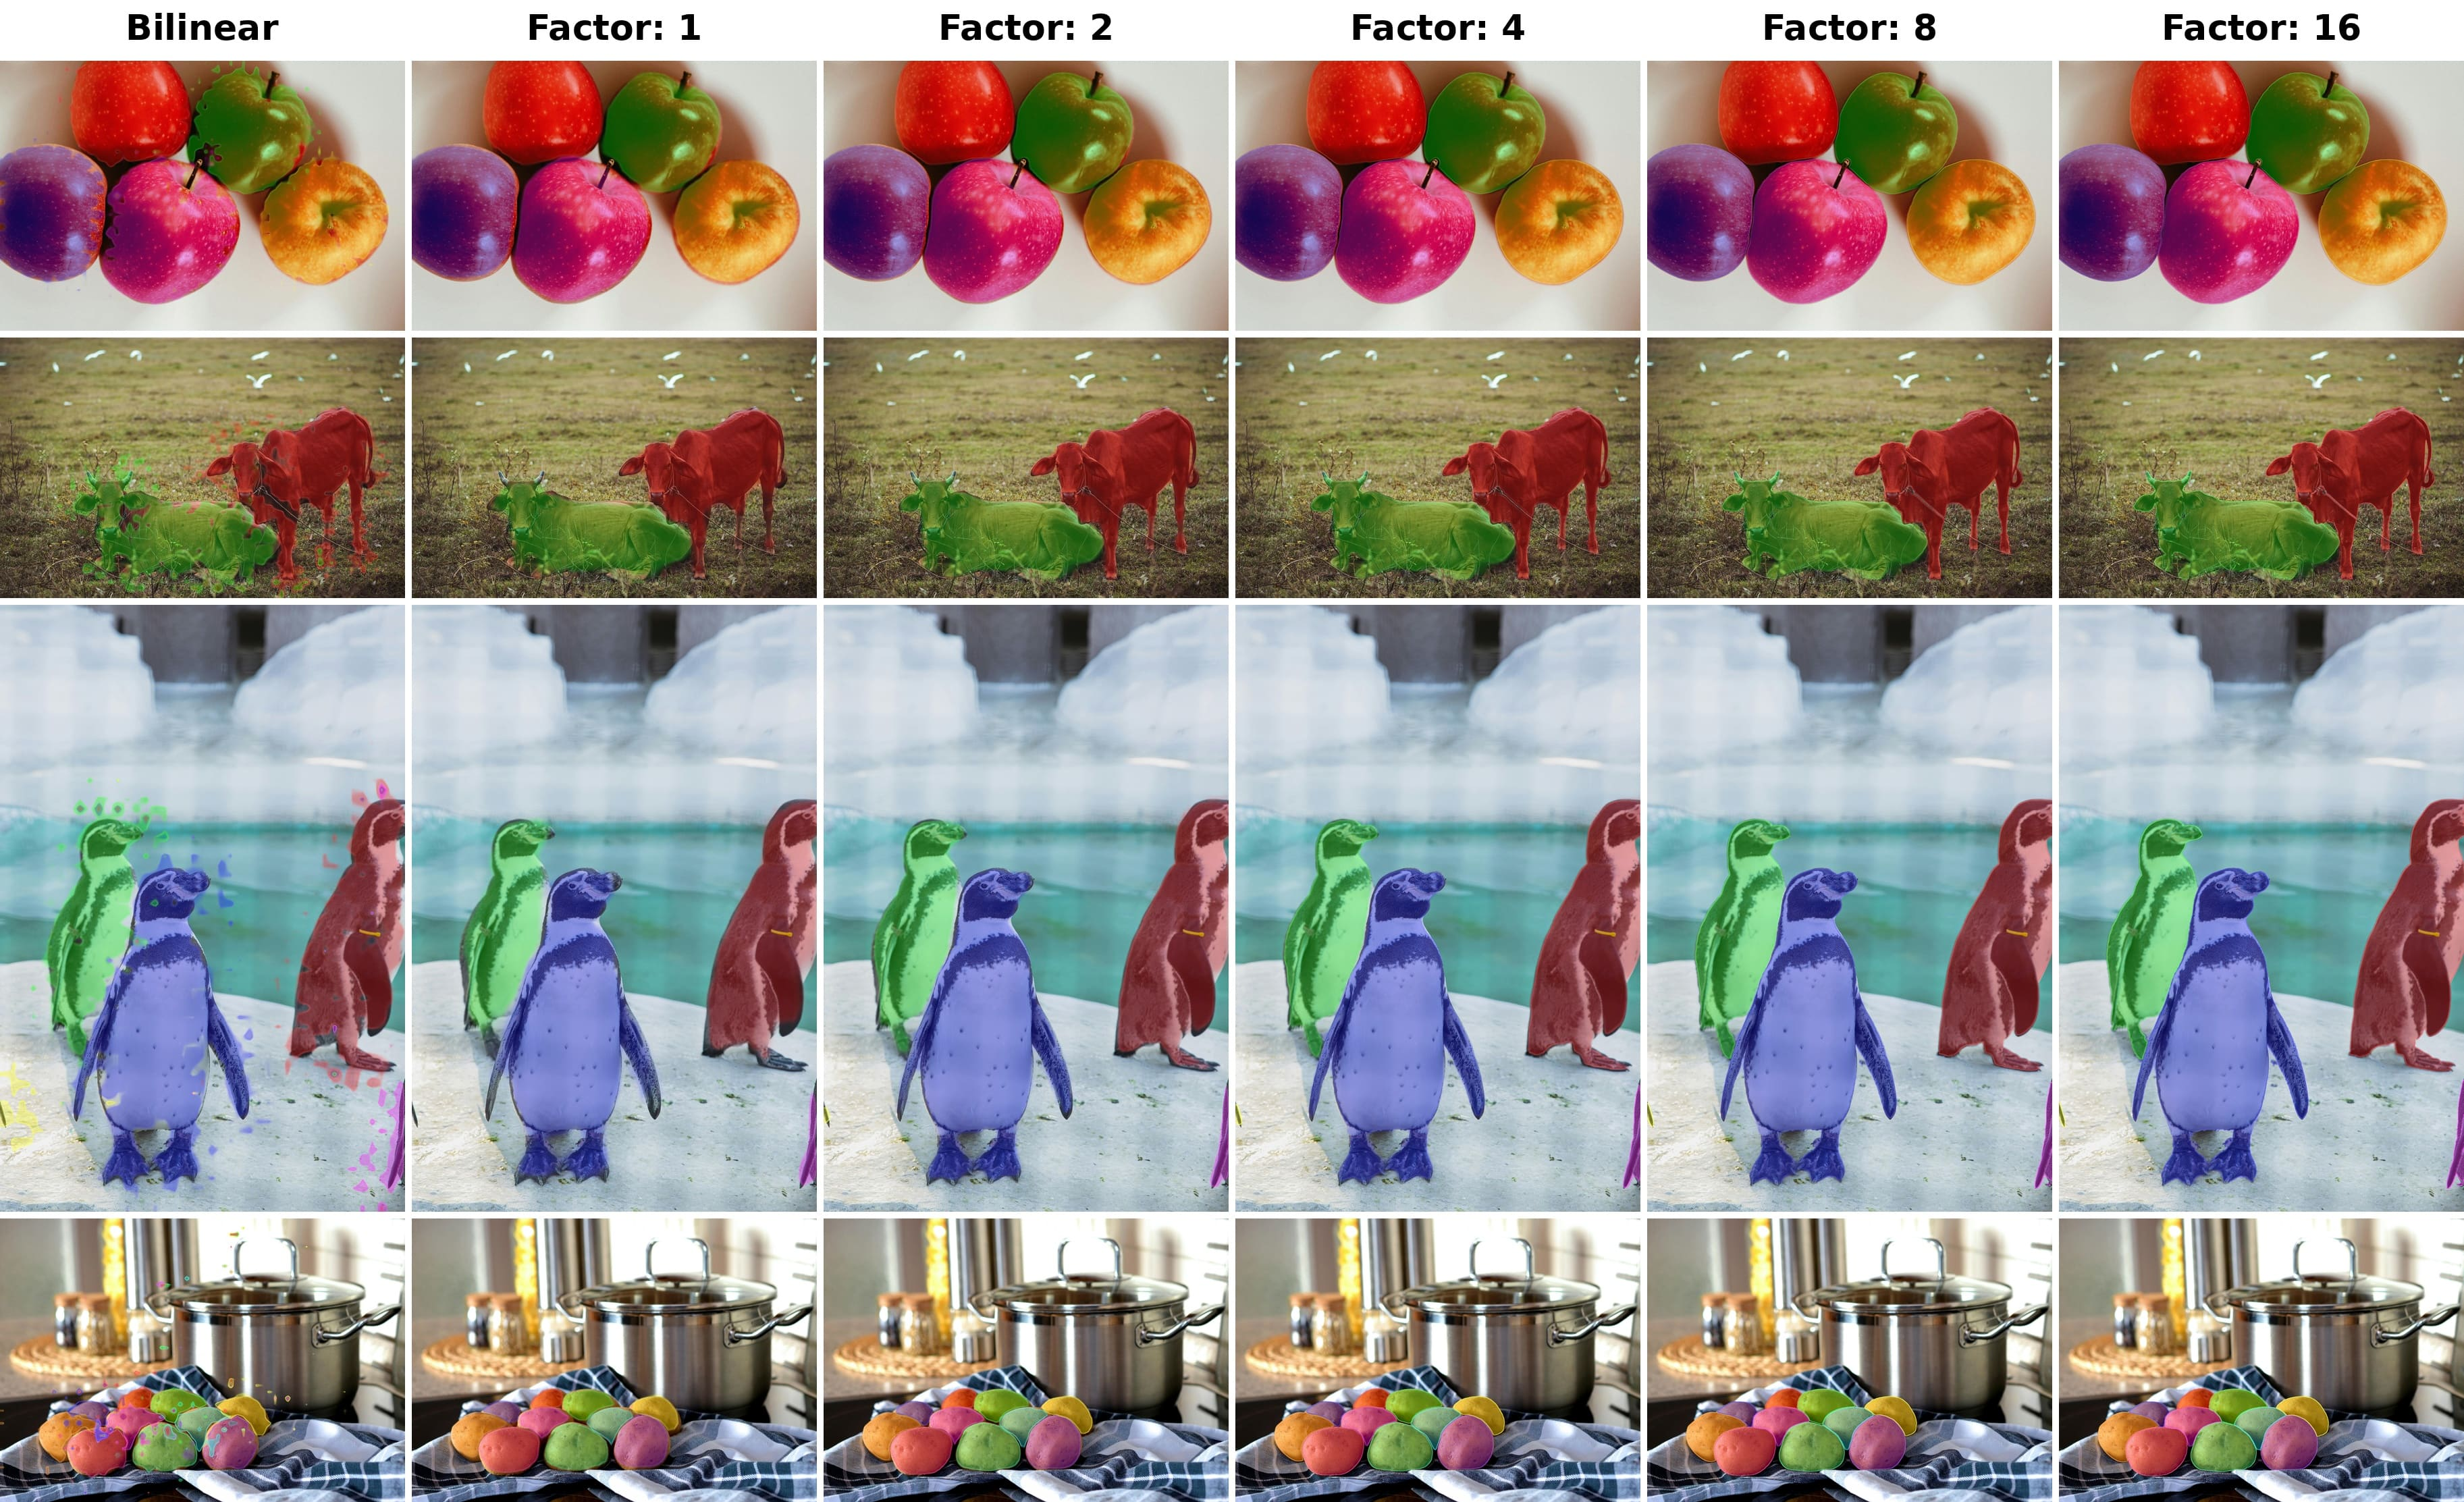
\includegraphics[width=1.0\textwidth]{figures/factor_grid.jpg}\vspace{-0.2cm}
\caption{\textbf{Impact of the upsampling factor during inference:} Bilinearly upsampling the image features at the perception model output (16x downsampled) and computing the instance masks results in degraded quality (leftmost column) with holes inside the instances and mask regions outside the instances. Processing the model output via the Anyup upsampler with different upsampling factors, followed by mask computation and bilinear upsampling of mask to image size significantly improves the mask quality (columns 2 to 6). Particularly, as the Anyup upsampling factor is increased, the instance boundaries are better refined. \Eg, in the top row, the boundaries of the fourth apple instance from left improves as the factor increases to 8 and 16. Similarly, in the third row, the beak of left penguin is incomplete for factors 1 to 4, while it is accurate for higher factors.\vspace{-0.2cm}}
\label{fig:appendix_impact_factor}
\end{figure}



\subsection{Qualitative Comparison with SAM 3}
Figures~\ref{fig:level_0}-\ref{fig:dense} show the qualitative comparison of the predicted masks between our Falcon Perception and SAM~3\footnote{While we acknowledge that SAM~3 cannot reliably predict masks for levels 2 to 4 since it is not trained in that manner, we compare with it to showcase the added capability of our Falcon Perception in this regard.} on various image-prompt pairs with  prompts varying from Level 0 to 4.  Overall, SAM 3 incorrectly predicts false positives when query prompts requiring visual text recognition (Figure~\ref{fig:level_2}), complex expression prompts are used (Figures~\ref{fig:level_3} and ~\ref{fig:level_4}) and is limited by the number of query tokens in its DETR decoder for dense predictions (Figure~\ref{fig:dense}). In contrast, our Falcon Perception can read text reasonably well, decipher complex expressions and predict the correct instances among other distractors in the scene. Furthermore, since our model's predictions are autoregressive in nature, once trained with such long-contexts, it can easily scale the detections to many instances (up to 600). These results show the added capabilities for our dense transformer based early-fusion perception model. 
\begin{figure}[!t]
  \centering
  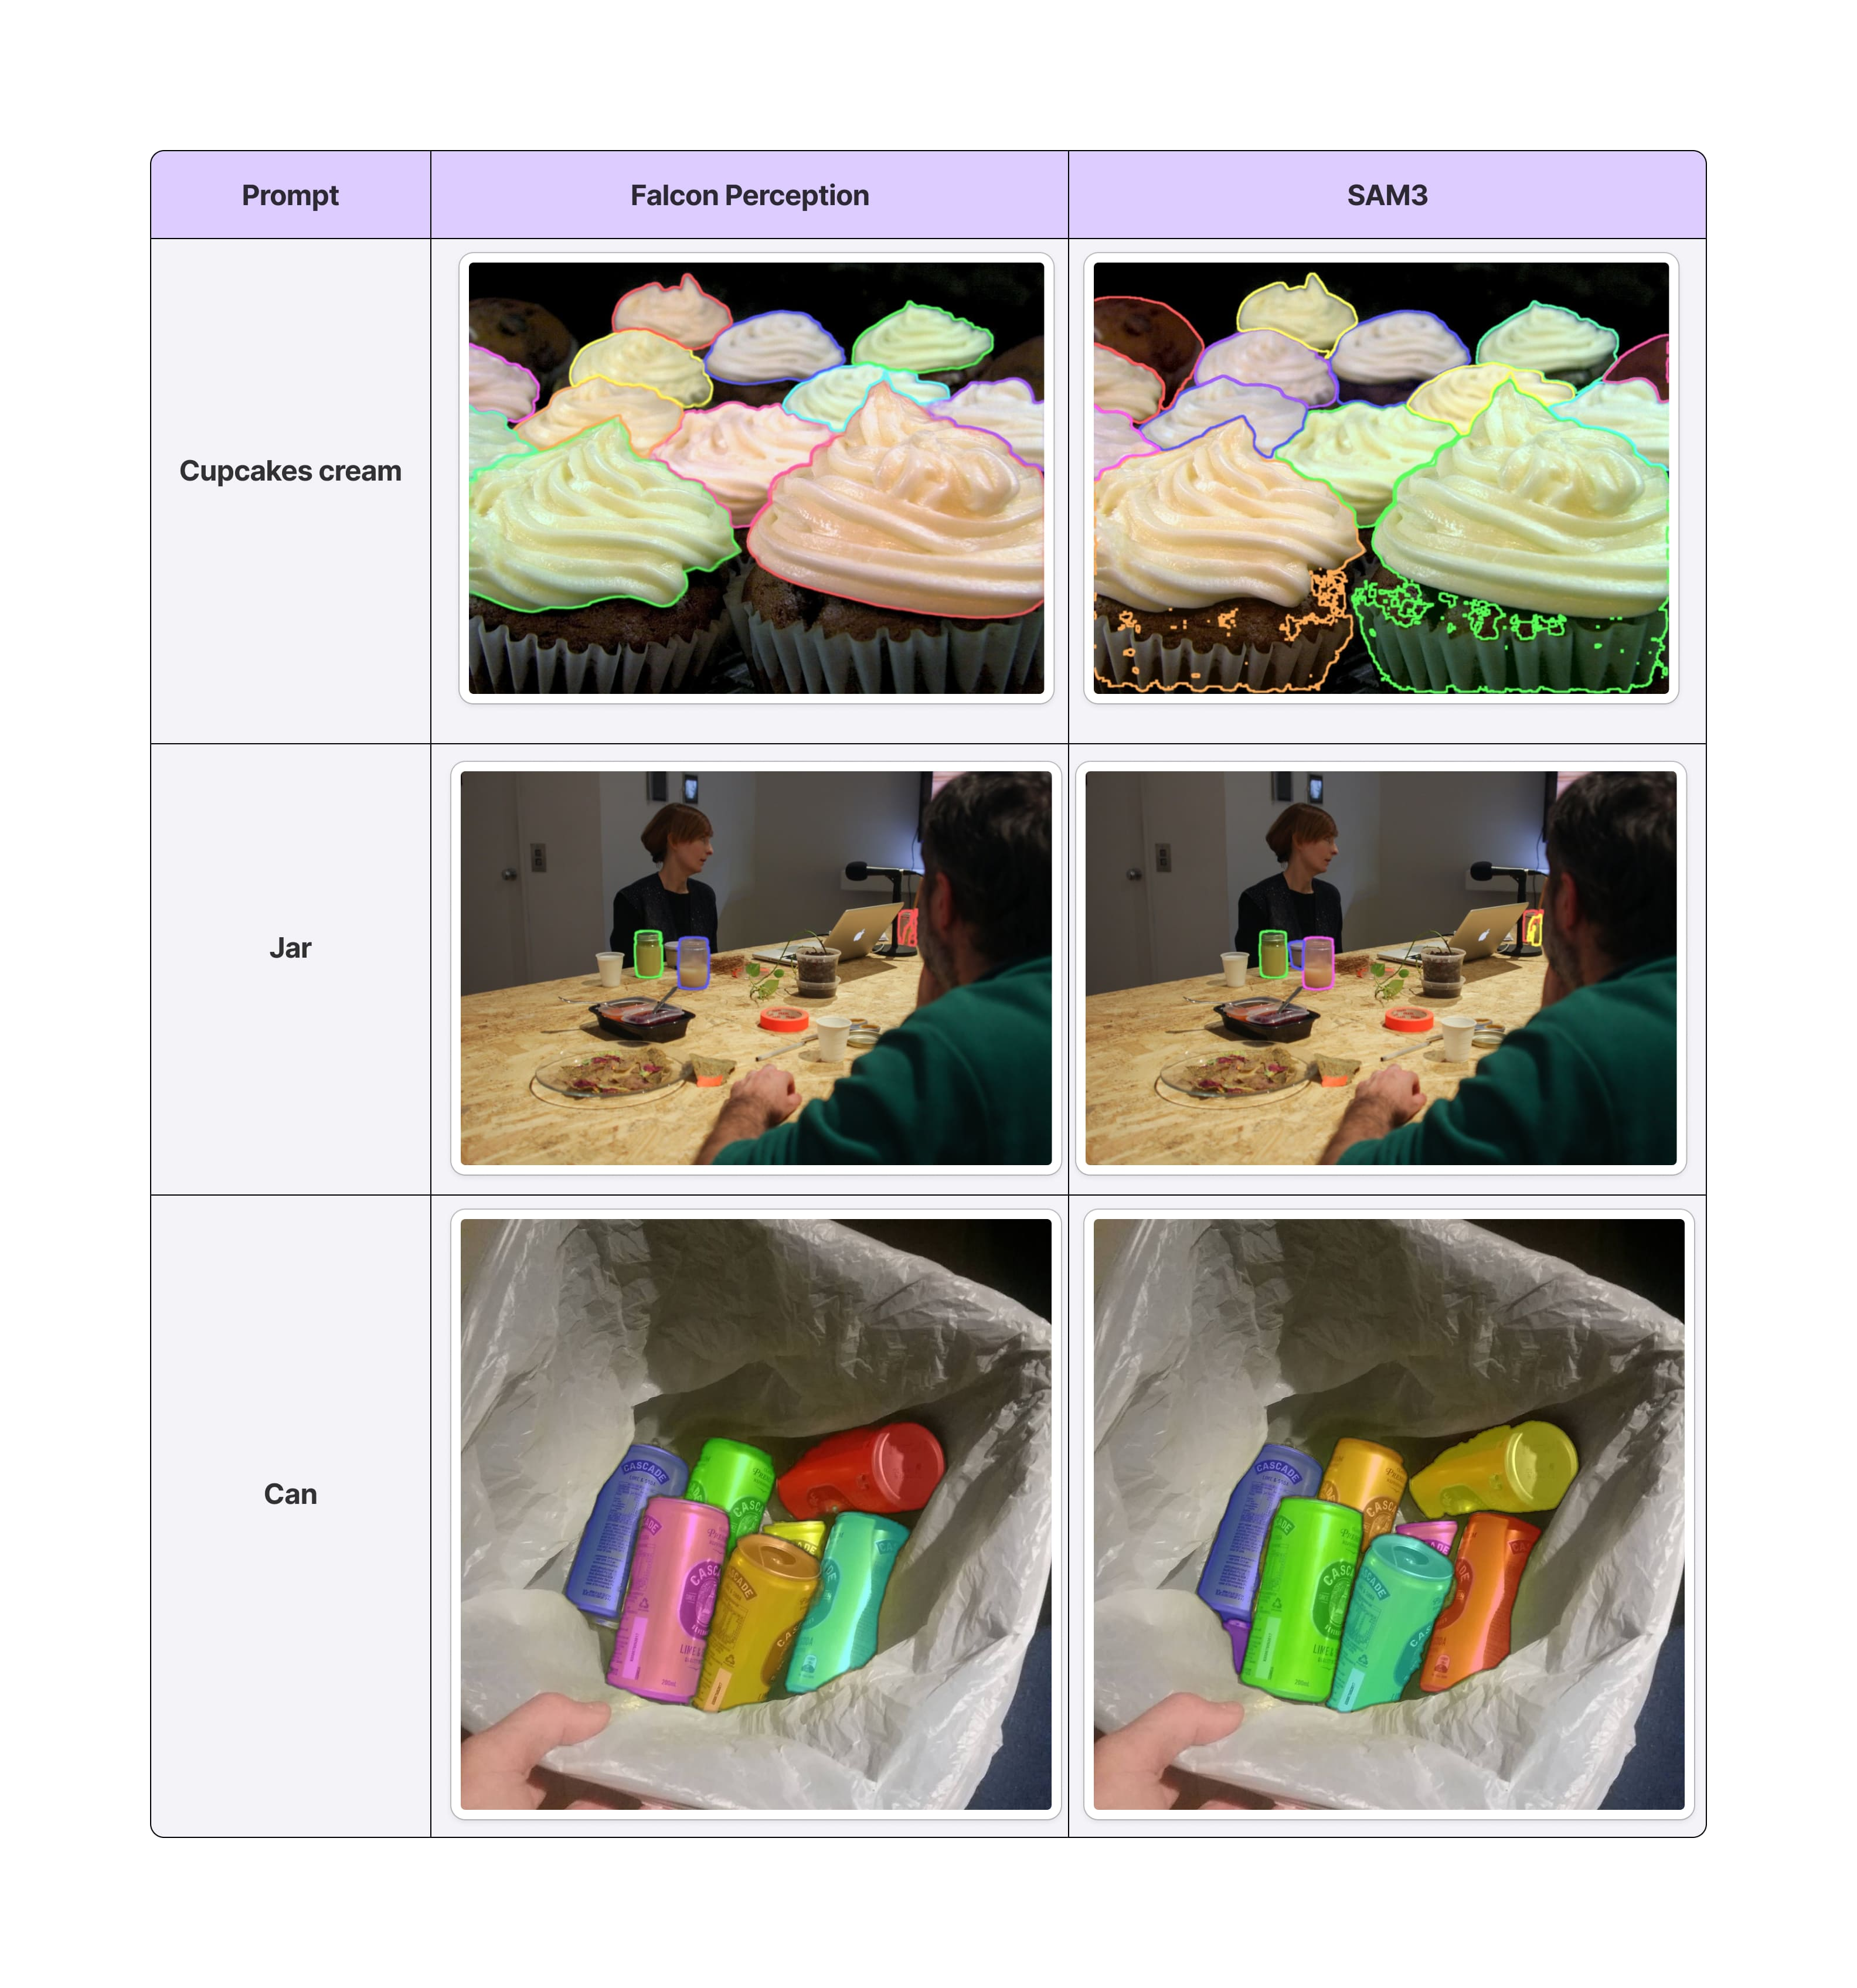
\includegraphics[width=\textwidth, trim=9cm 9cm 9cm 9cm, clip]{figures/level_0.jpg}
  \caption{\textbf{Level 0:} While our Falcon Perception predicts correct masks, SAM 3 incorrectly predicts cupcakes in the masks for the \textit{cupcakes cream} example on top row and an additional \textit{jar} in the middle (middle row).\vspace{-0.5cm}}
  \label{fig:level_0}
\end{figure}


\begin{figure}[t]
  \centering
  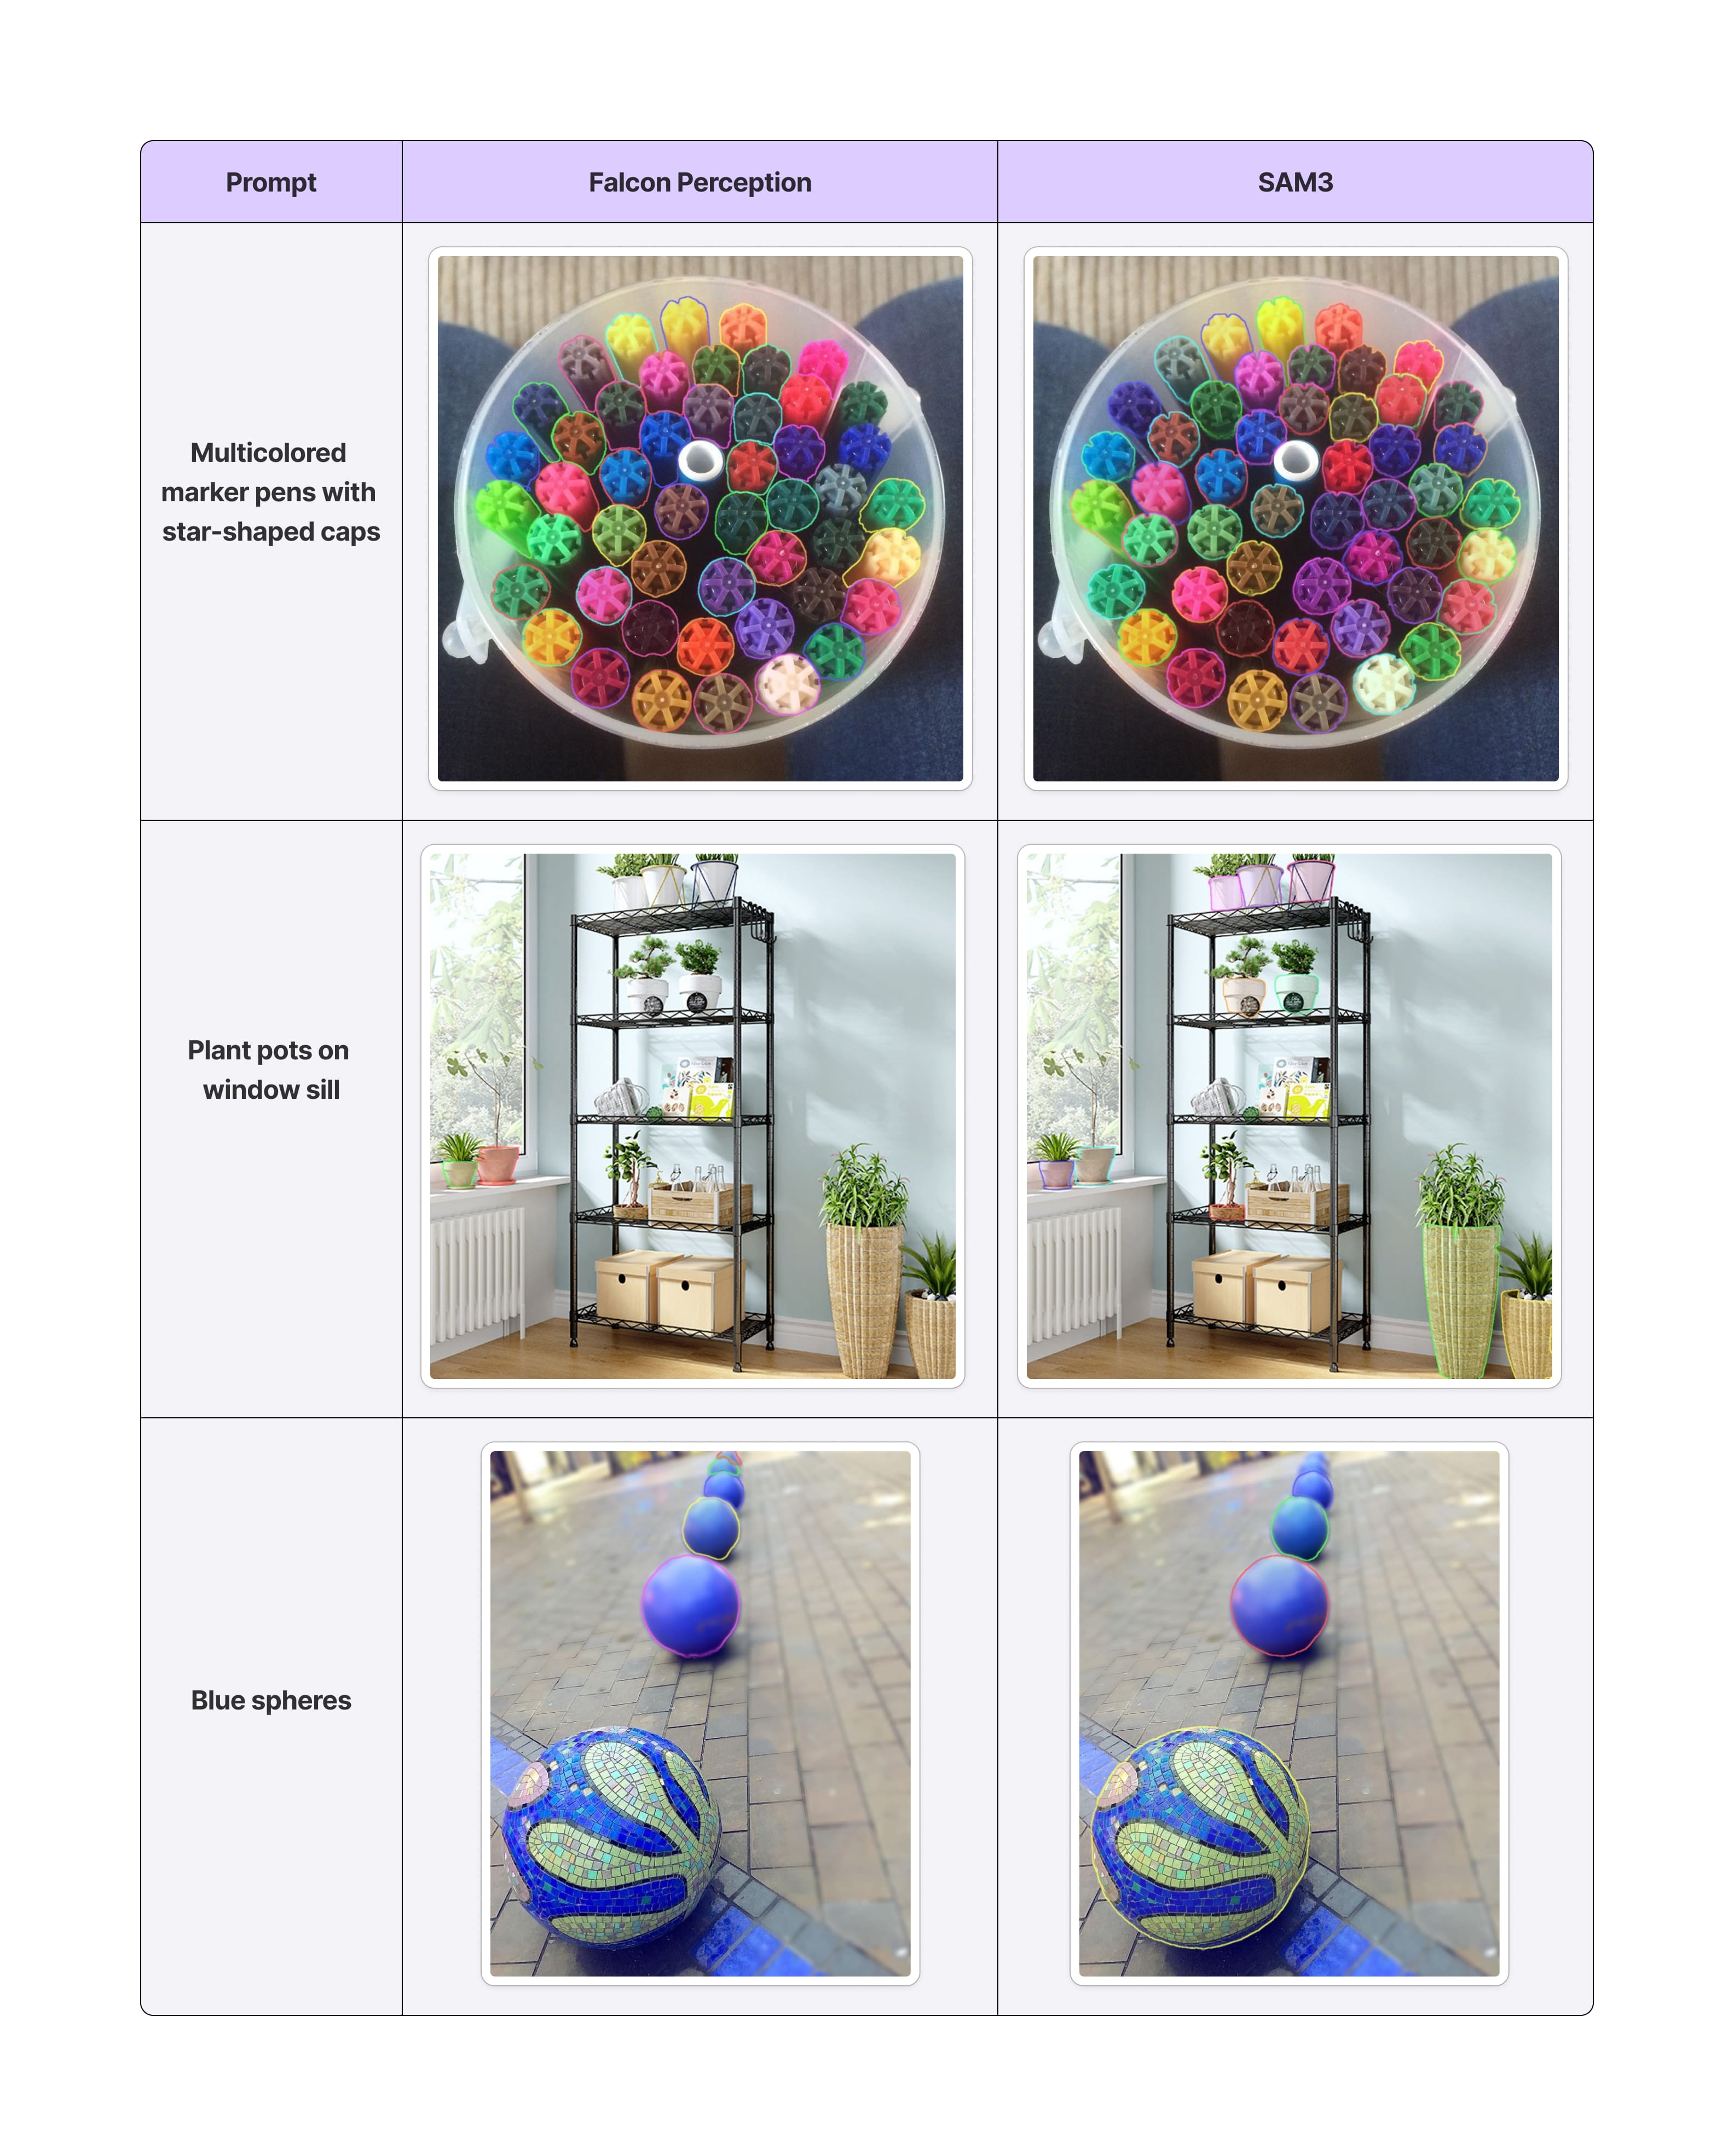
\includegraphics[width=1.0\textwidth, trim=9cm 9cm 9cm 9cm, clip]{figures/level_1.jpg}
  \caption{\textbf{Level 1:} Our Falcon perception misses few marker pens in the top row, clearly distinguishes the plant pots on the window sill from the other plant pots in the middle row. In contrast, SAM 3 identifies all the marker pens correctly but fails to distinguish between plant pots in the middle row by predicting false positives for pots not placed on window sill.}
  \label{fig:level_1}
\end{figure}


\begin{figure}[t]
  \centering
  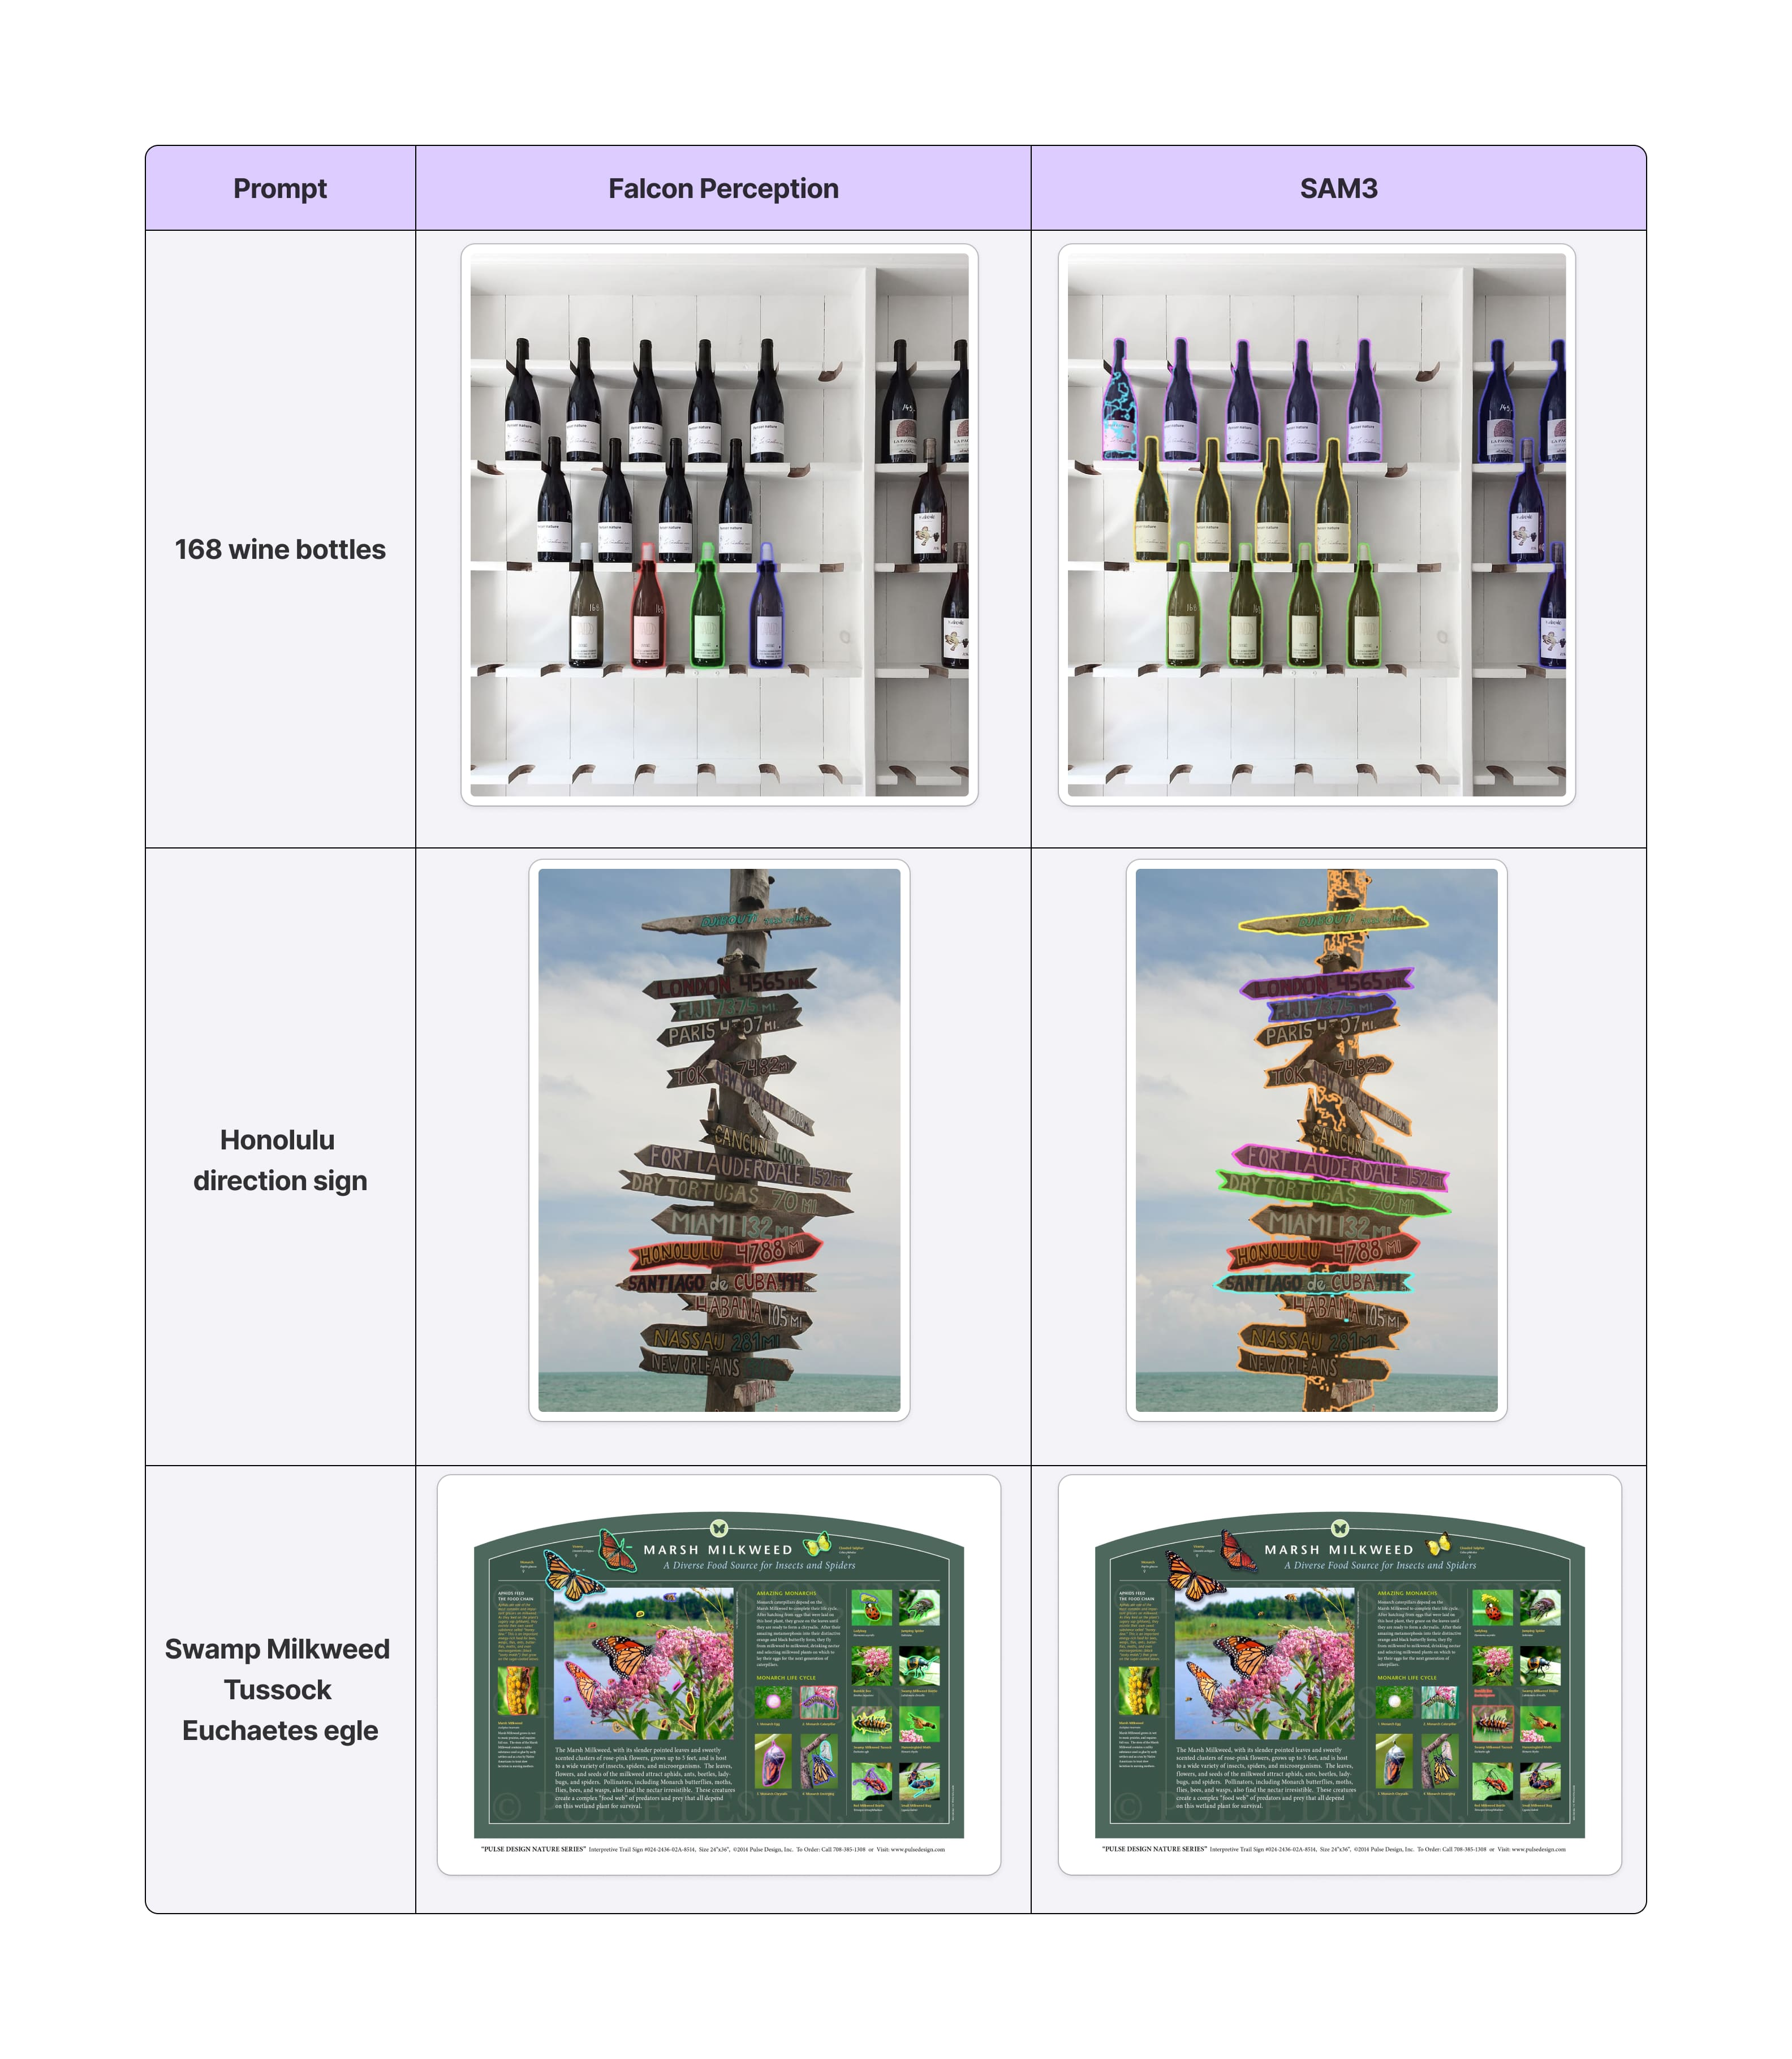
\includegraphics[width=1.0\textwidth, trim=9cm 9cm 9cm 9cm, clip]{figures/level_2.jpg}
  \caption{\textbf{Level 2:} Different to SAM 3 that incorrectly predicts masks for each bottle (top row) and each sign (middle row), our Falcon Perception model correctly identifies the \textit{168 wine bottles} (marked with 168) and the \textit{Honolulu direction sign}, indicating that our model can better relate the query prompt to the OCR text in the image. }
  \label{fig:level_2}
\end{figure}


\begin{figure}[t]
  \centering
  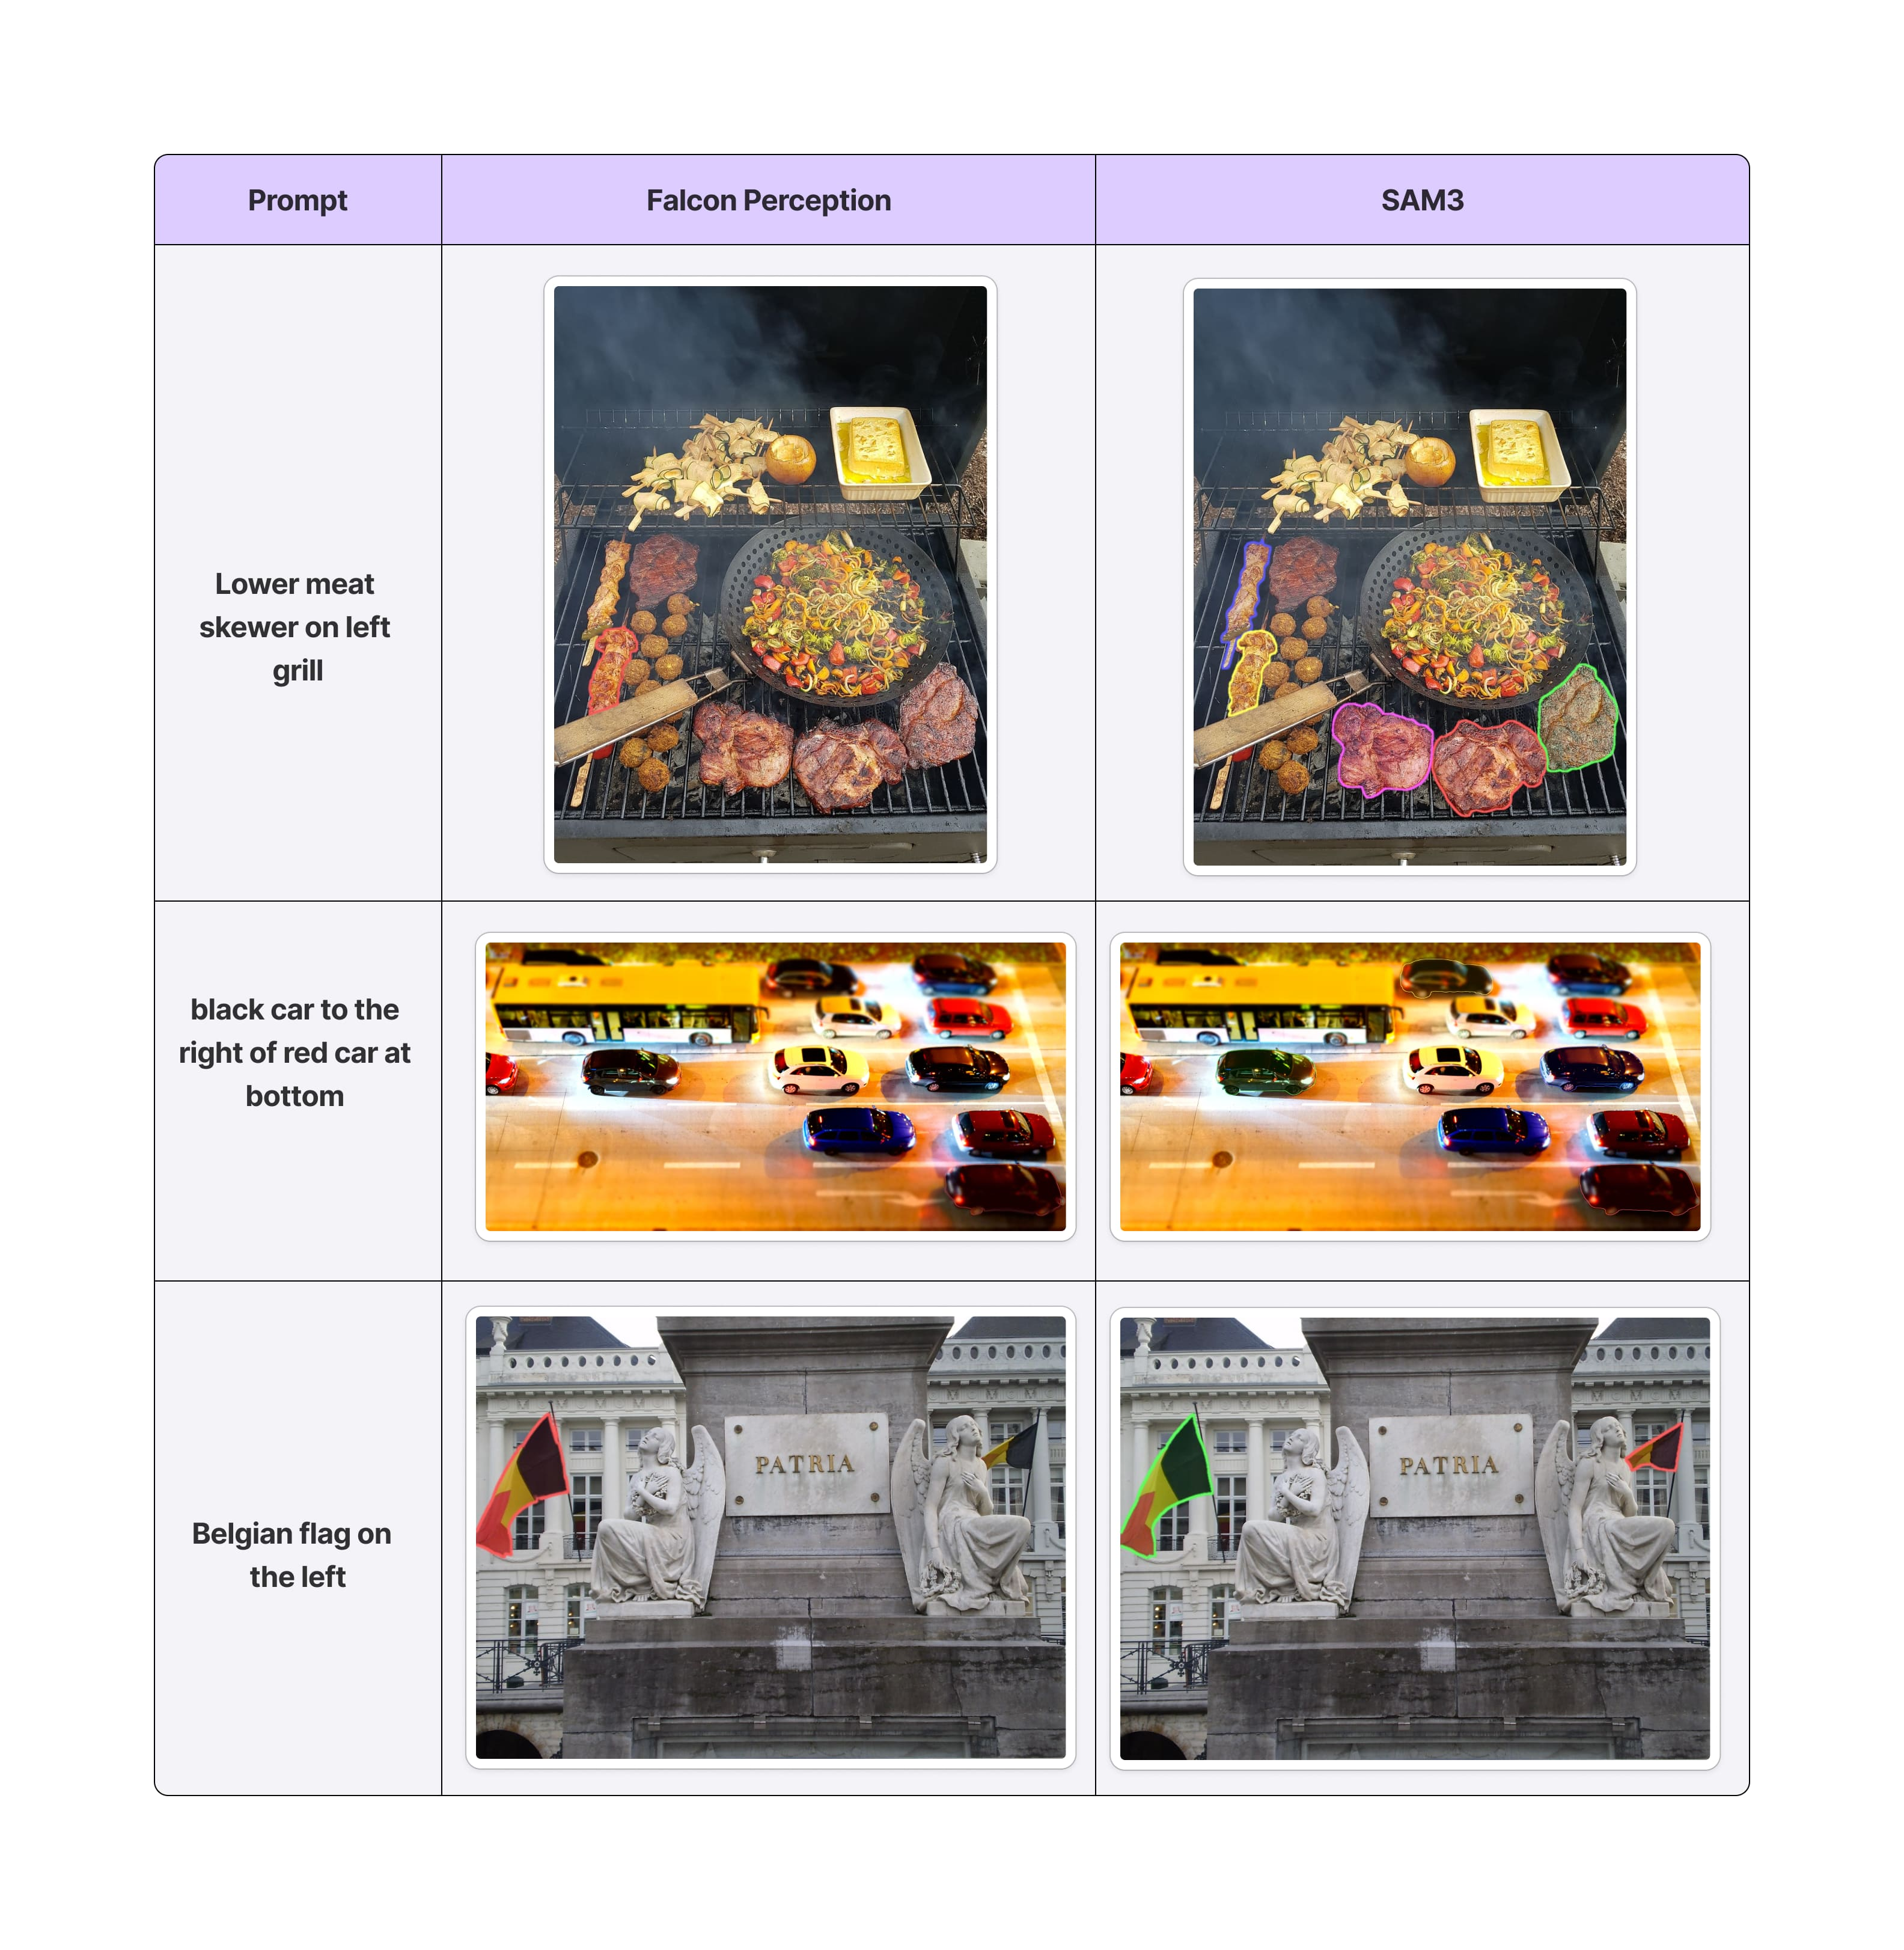
\includegraphics[width=1.0\textwidth, trim=9cm 9cm 9cm 9cm, clip]{figures/level_3.jpg}
  \caption{\textbf{Level 3:} In contrast to SAM 3 predicting false positives for meat (top row), black car (middle row) and Belgian flag (bottom row), our model correctly identifies the \textit{lower meat skewer on left grill}, {black car to the right of red car at bottom} and \textit{Belgian flag on the left} in the three examples. This shows that our Falcon Perception has better spatial understanding of the scene.}
  \label{fig:level_3}
\end{figure}



\begin{figure}[t]
  \centering
  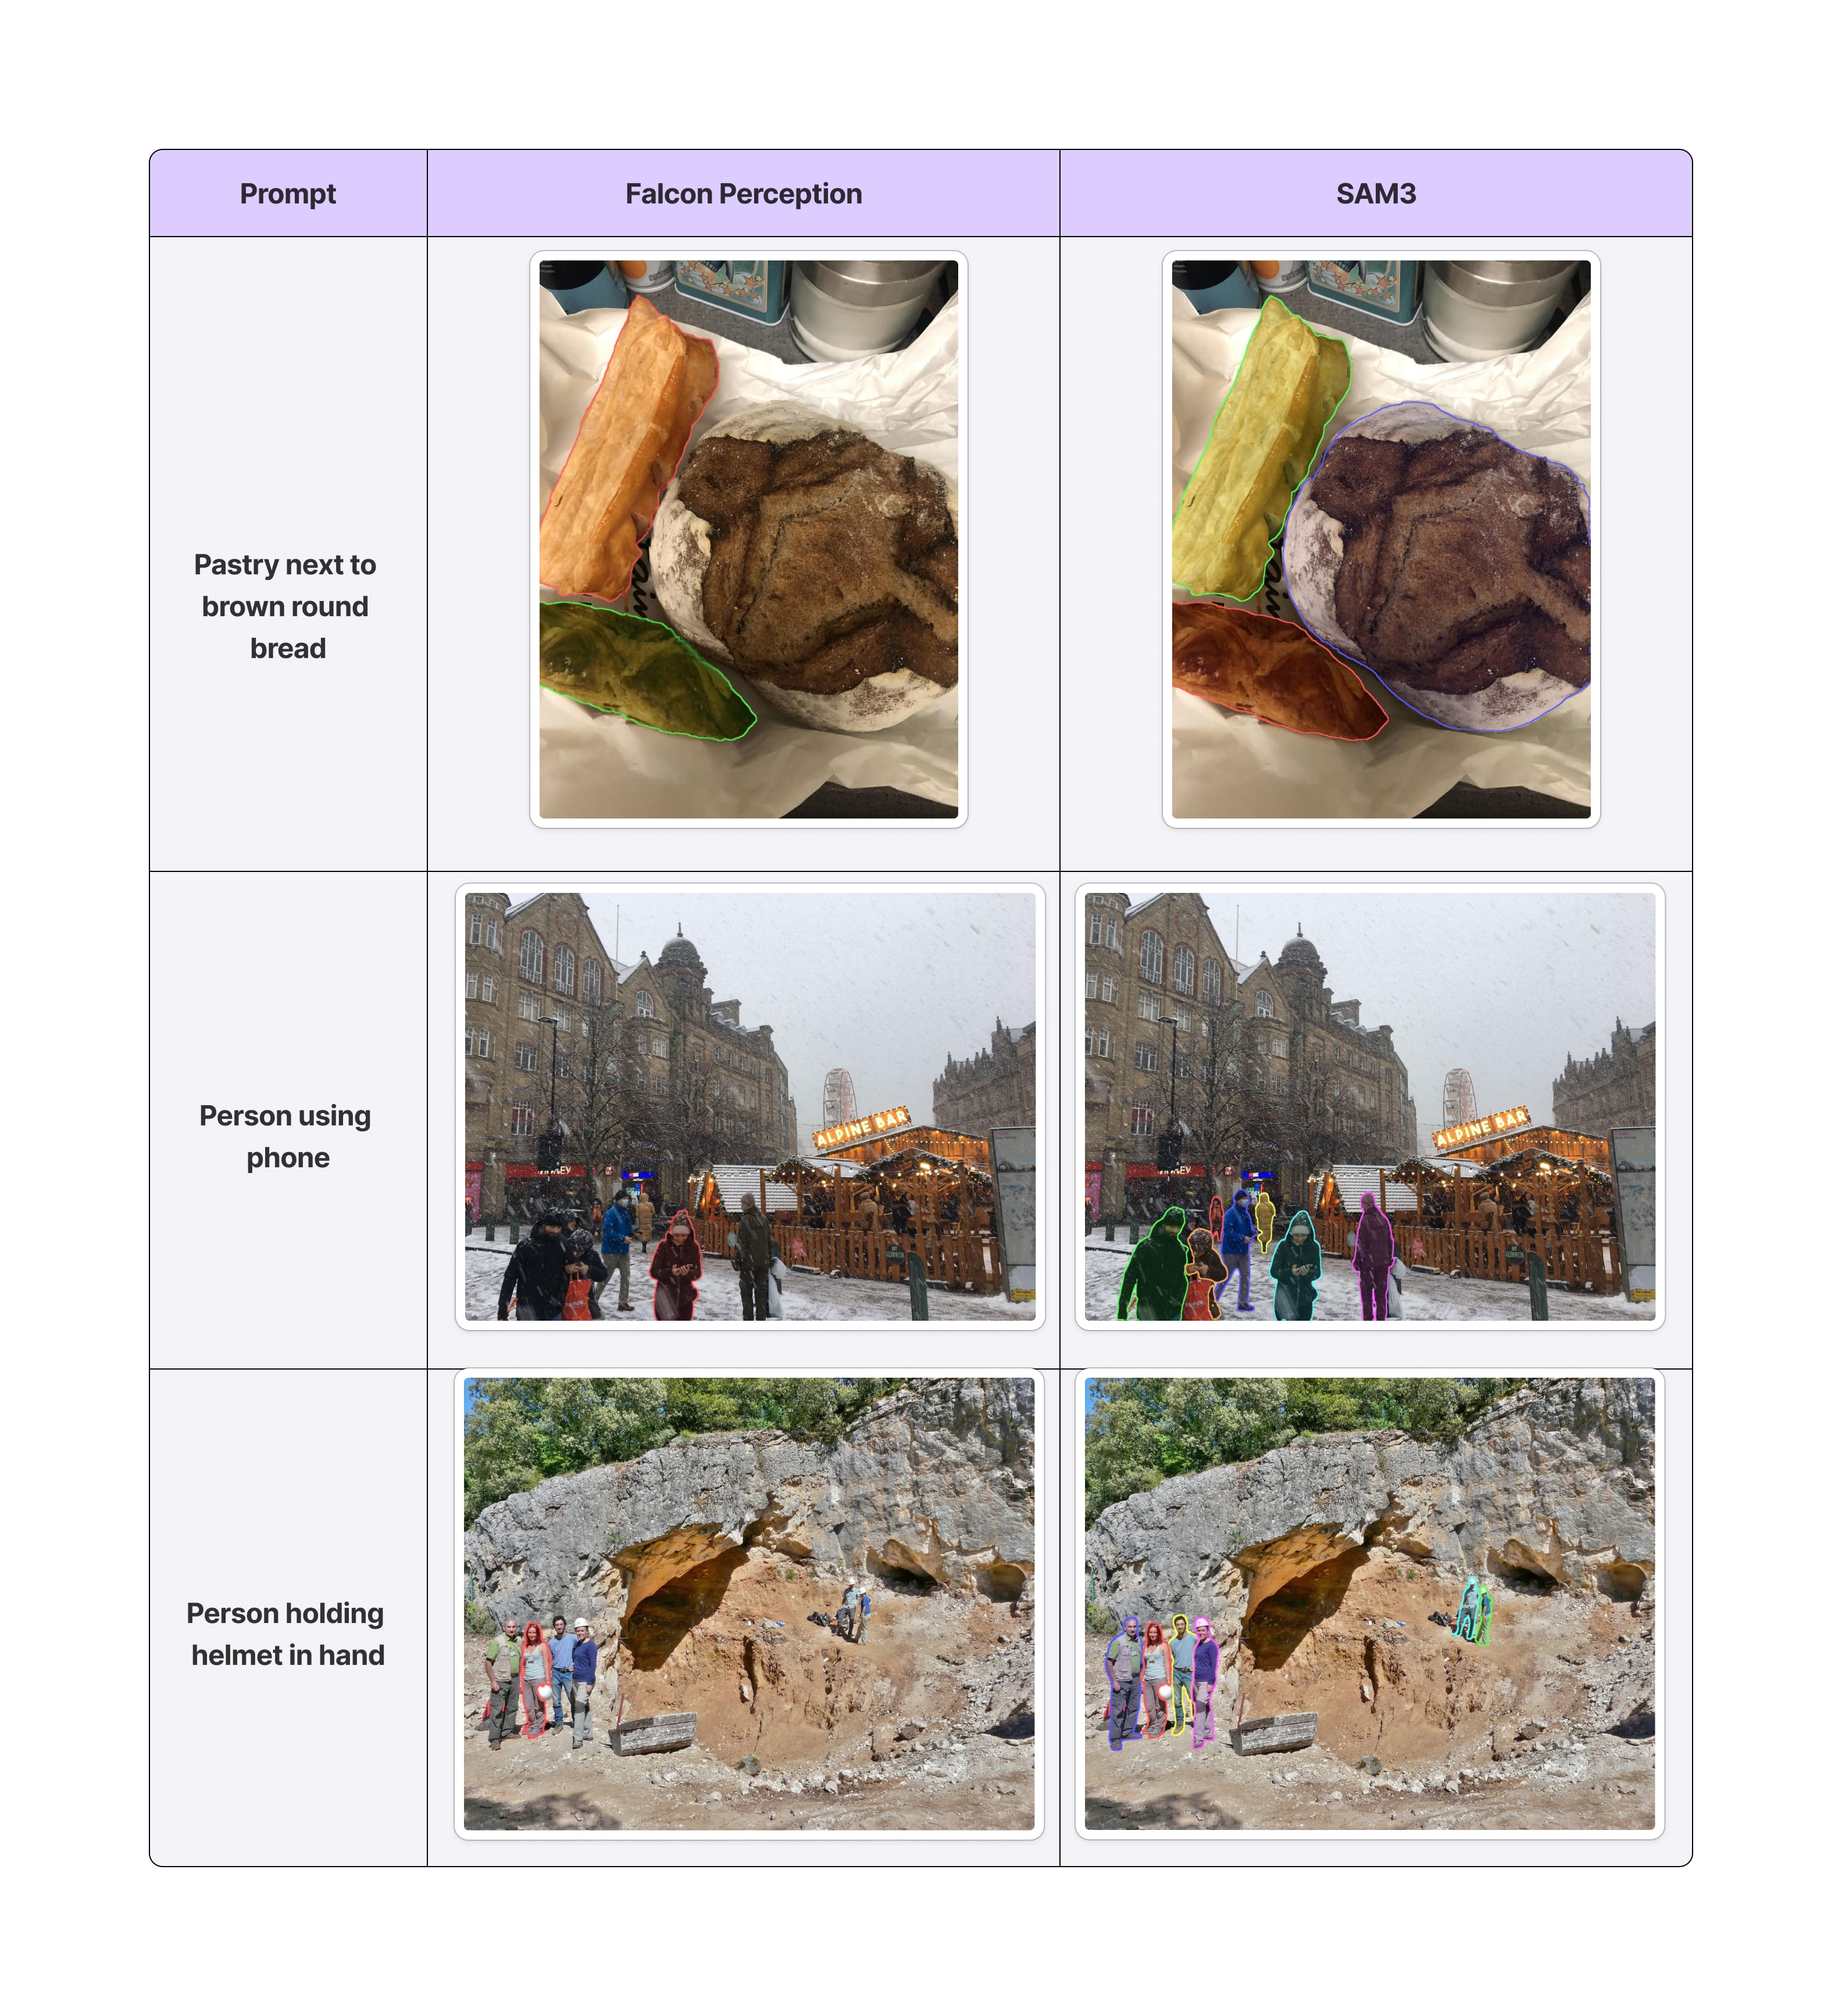
\includegraphics[width=1.0\textwidth, trim=9cm 9cm 9cm 9cm, clip]{figures/level_4.jpg}
  \caption{\textbf{Level 4:} SAM 3 wrongly outputs masks for all bread (top row), persons (middle and bottom rows). However, our Falcon Perception model correctly identifies the object instances for \textit{pastry next to brown round bread}, \textit{person holding phone} and \textit{person holding helmet in hand}, thereby showcasing the ability to understand the object interaction in the scene.}
  \label{fig:level_4}
\end{figure}


\begin{figure}[t]
  \centering
  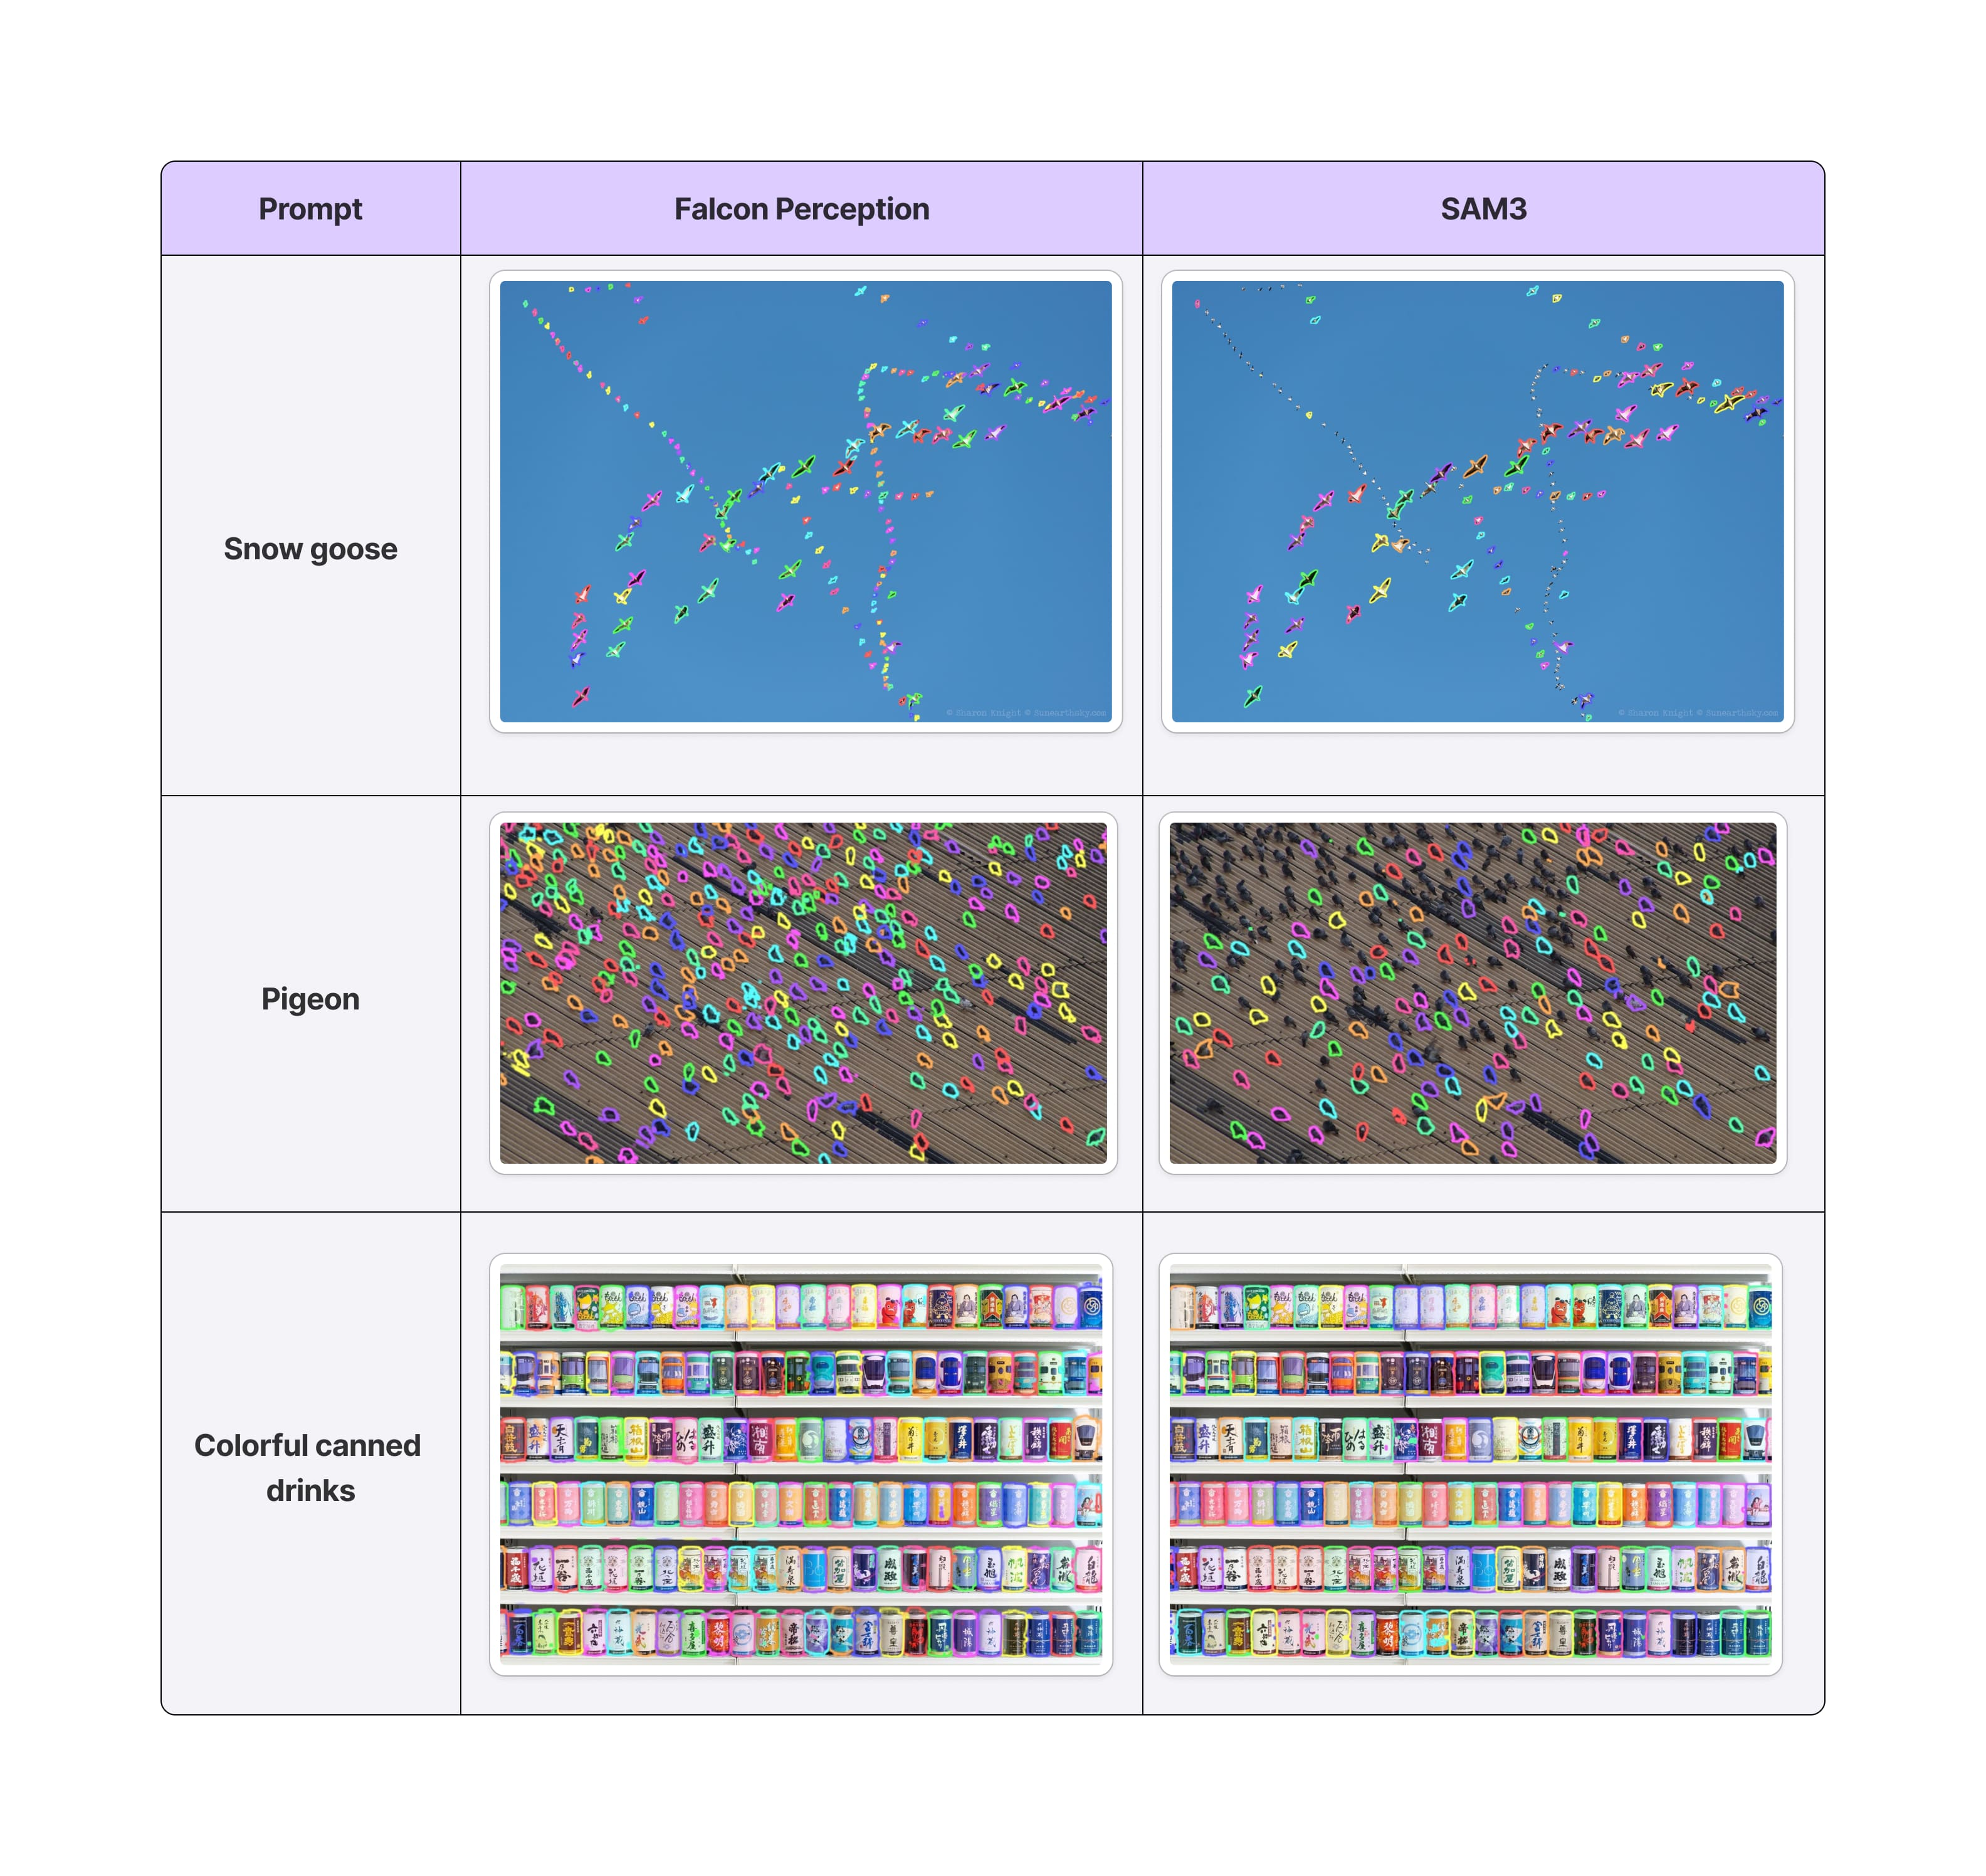
\includegraphics[width=1.0\textwidth, trim=9cm 9cm 9cm 9cm, clip]{figures/dense.jpg}
  \caption{\textbf{Dense Split:} While SAM 3 is capable of identifying many instances of an object, it fails to predict masks when number of instances exceeds 200 due to the fixed number of query tokens in the decoder. Our Falcon Perception, following the autoregressive approach for prediction, is not limited by this and can easily scale higher, as shown for \textit{snow goose}, \textit{pigeon} and \textit{colorful canned drinks} in the three rows.}
  \label{fig:dense}
\end{figure}

\subsection{Effect of Sampling\label{sec:appendix_sampling}}
Figure~\ref{appendix:sampling} shows the effect of sampling tokens, center, and size with higher temperature, compared to greedy sampling. We observe that the quality of predictions improves with non-deterministic sampling (\eg, \textit{reflection of person} in the 2$^{nd}$ row) and even smaller scale instances are identified (\eg, \textit{truck on road} in the 3$^{rd}$ row). This, along with the results in Section~\ref{sec:sampling} shows that our model has the required reasoning to predict the instances correctly, and with RL-style post-training, it can perform better.

\begin{figure}[t]
  \centering
  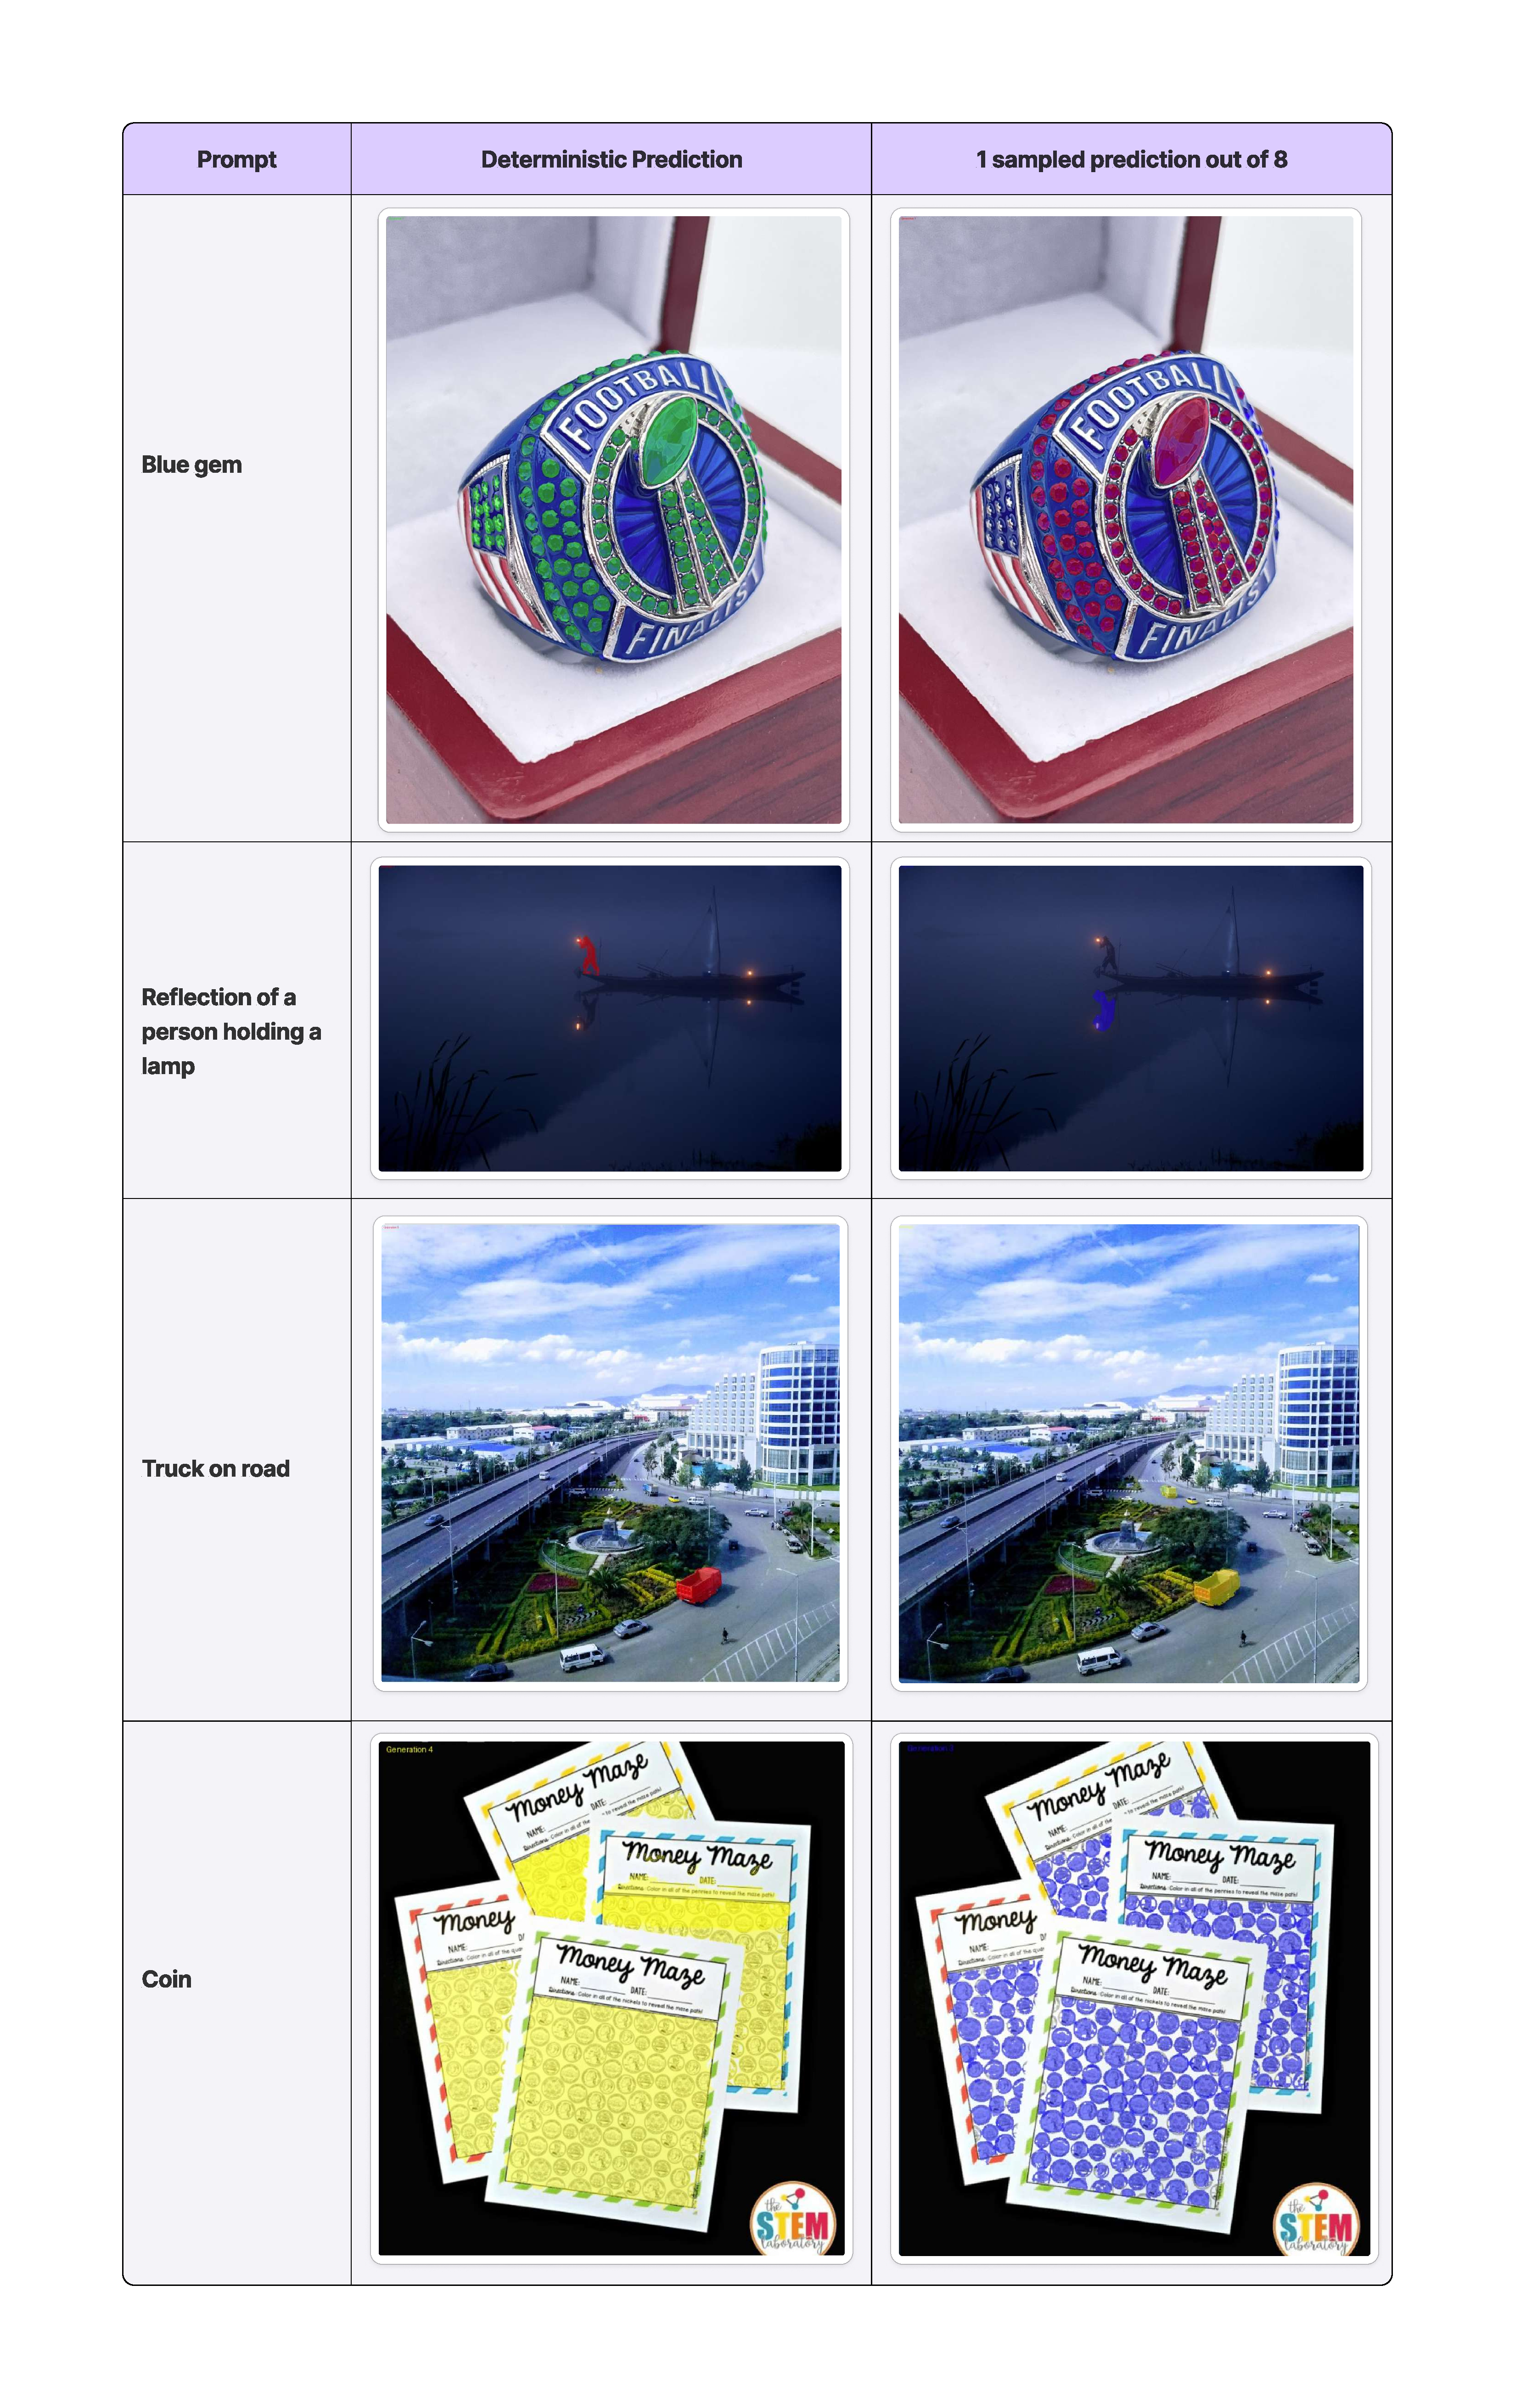
\includegraphics[height=0.88\textheight, trim=4.5cm 4.5cm 4.5cm 4.5cm, clip]{figures/sampling/qualitative_examples.pdf}
  \caption{\textbf{Effect of sampling on the quality of predictions:} In the left column, we show the deterministic predictions, selecting the most likely next token, center coordinate, or size value. On the right, we show one of the predictions we obtain by sampling tokens, center, and size with a temperature of $0.7$. Oftentimes, we can achieve better predictions for instances that require reasoning over the query, fine-grained perception, and small or distant objects.}
  \label{appendix:sampling}
\end{figure}

\clearpage

\section{Qualitative Analysis - OCR}
In this section, we provide some qualitative results, showcasing the capabilities and some failure cases of our FalconOCR model. As seen from Figures~\ref{fig:paper2_ocr} to \ref{fig:tables}, our model ingests images taken in challenging real world conditions with challenging lighting and the text possessing differing semantics (formulas, tables, handwritten, etc) and output the proper structured text.
\begin{figure}[t!]
  \centering
  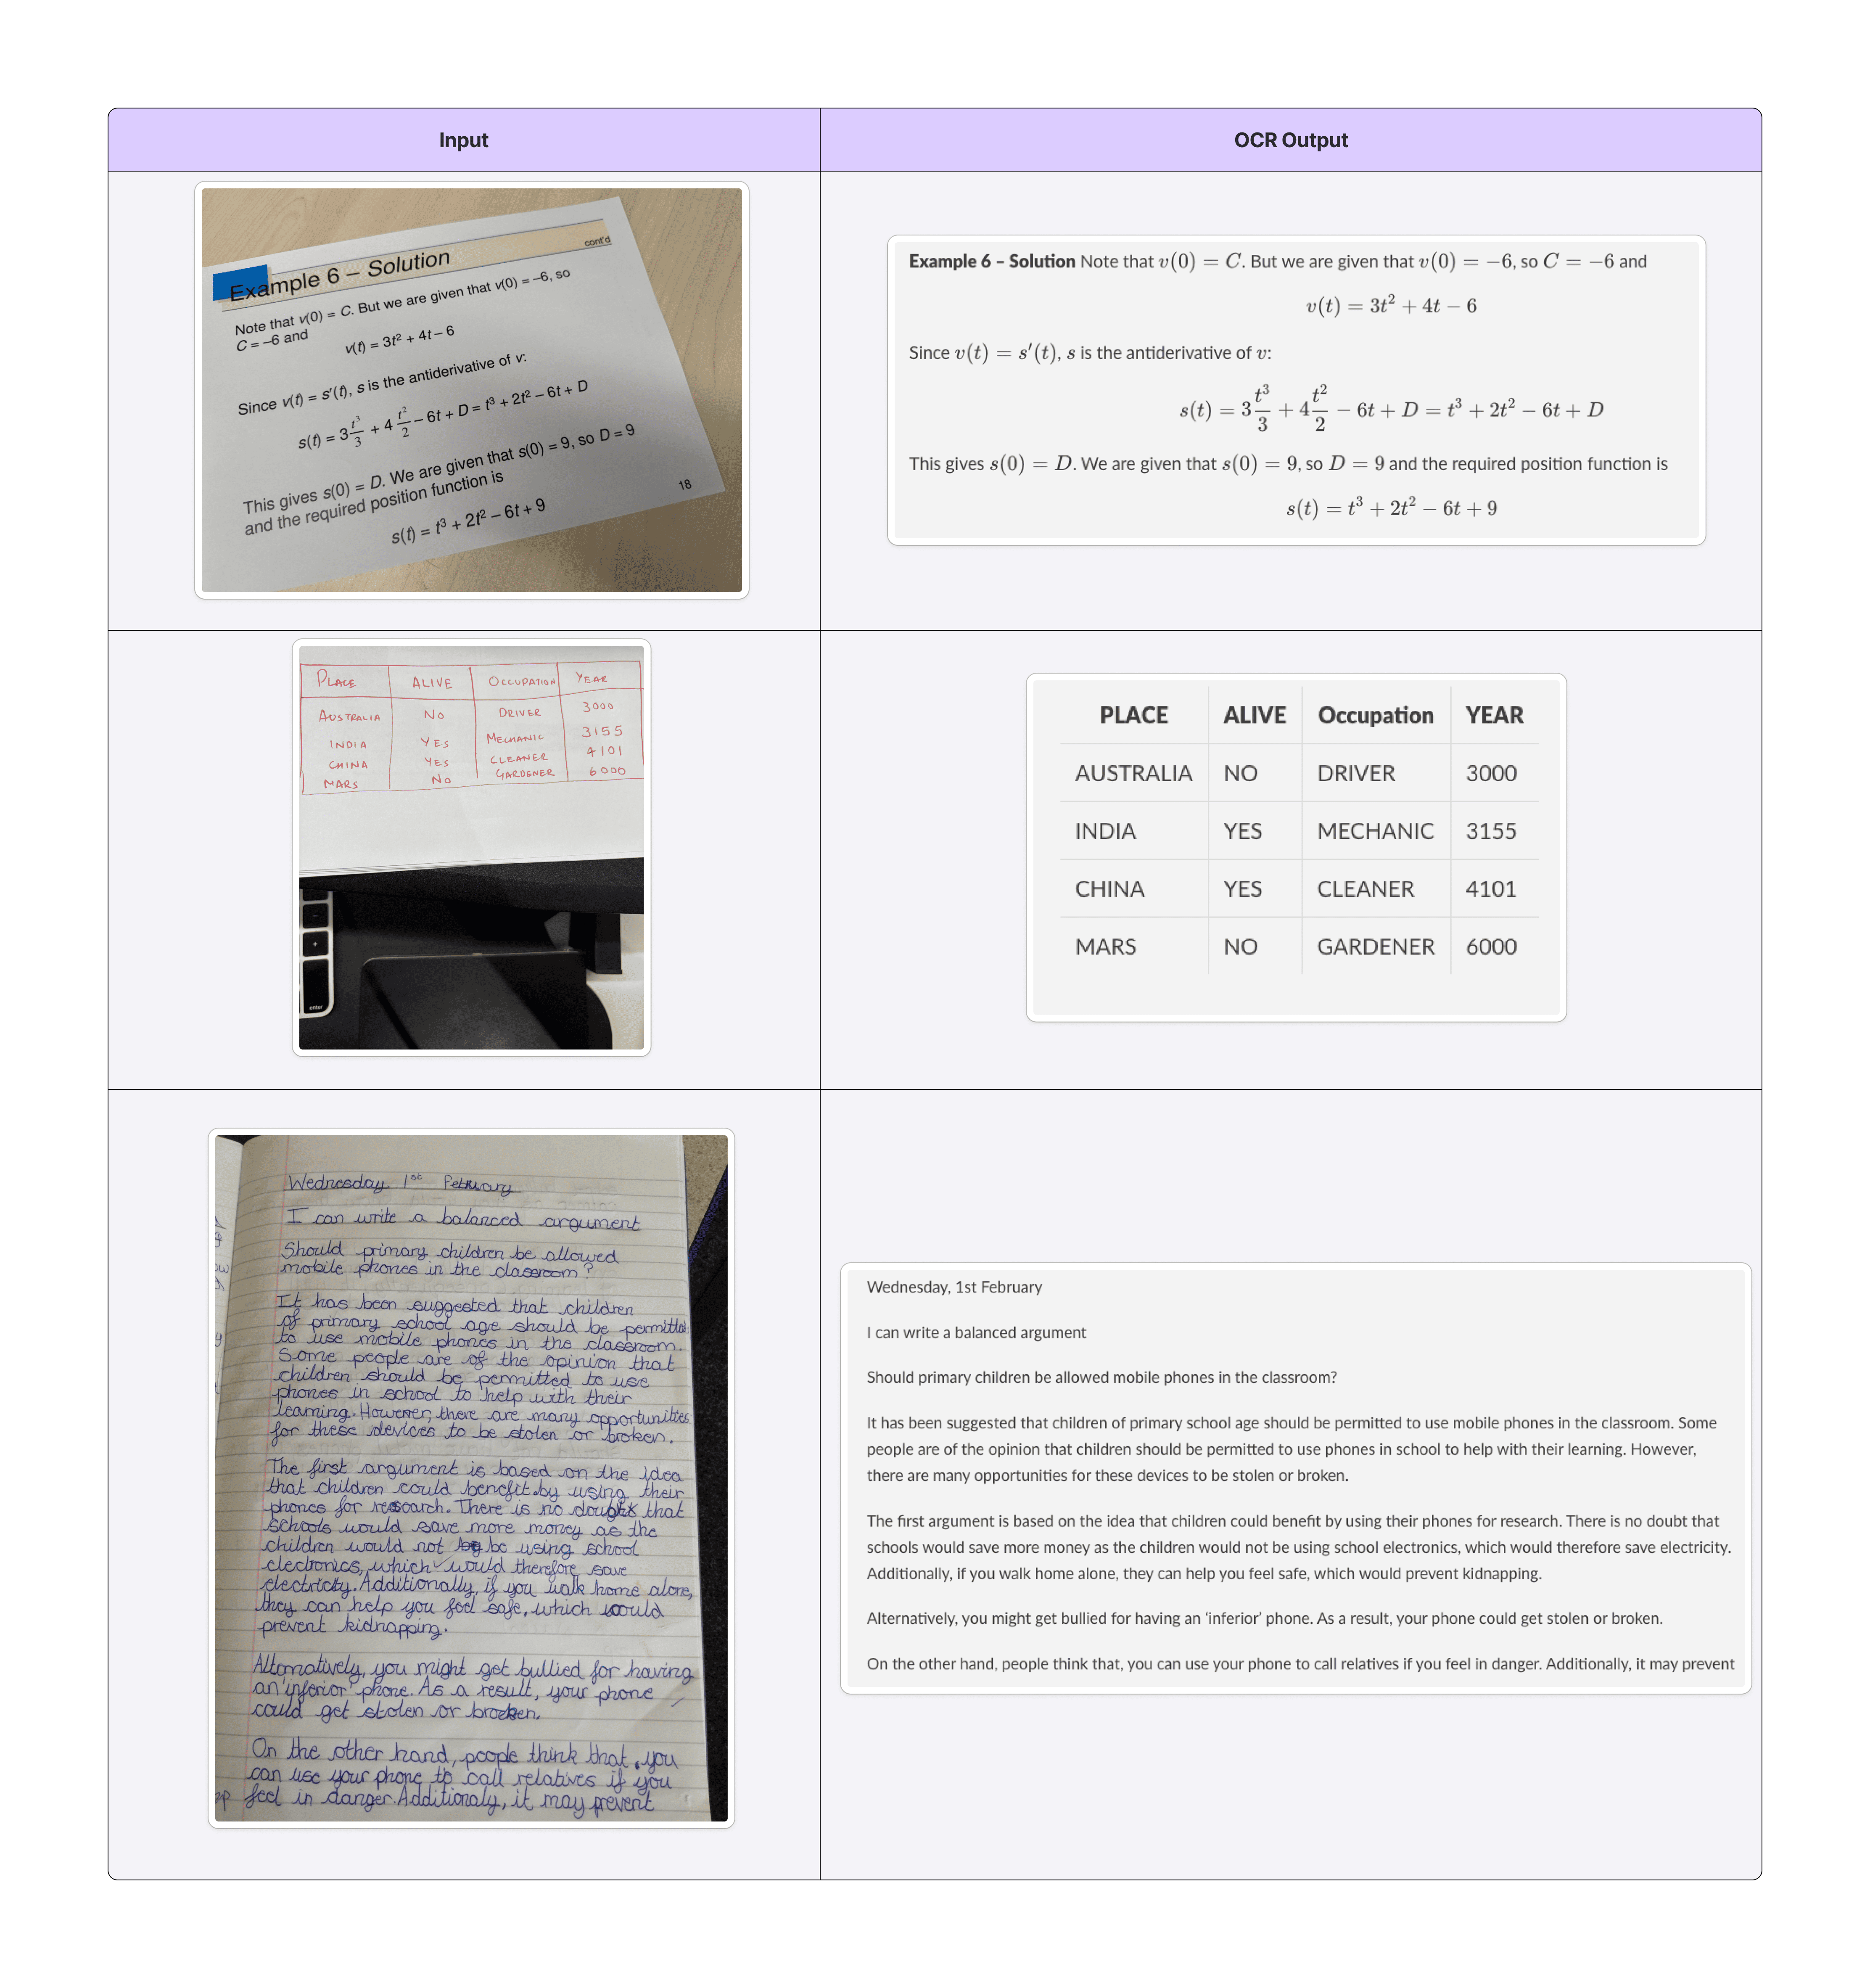
\includegraphics[width=1.0\textwidth, trim=4.5cm 4.5cm 4.5cm 4.5cm, clip]{figures/appendix_ocr/realworld.png}
  \caption{Example OCR output for inputs comprising formulae, tables and handwriting (from top to bottom). Best viewed zoomed-in.}
  \label{fig:realword_ocr}
\end{figure}



\begin{figure}[t!]
  \centering
  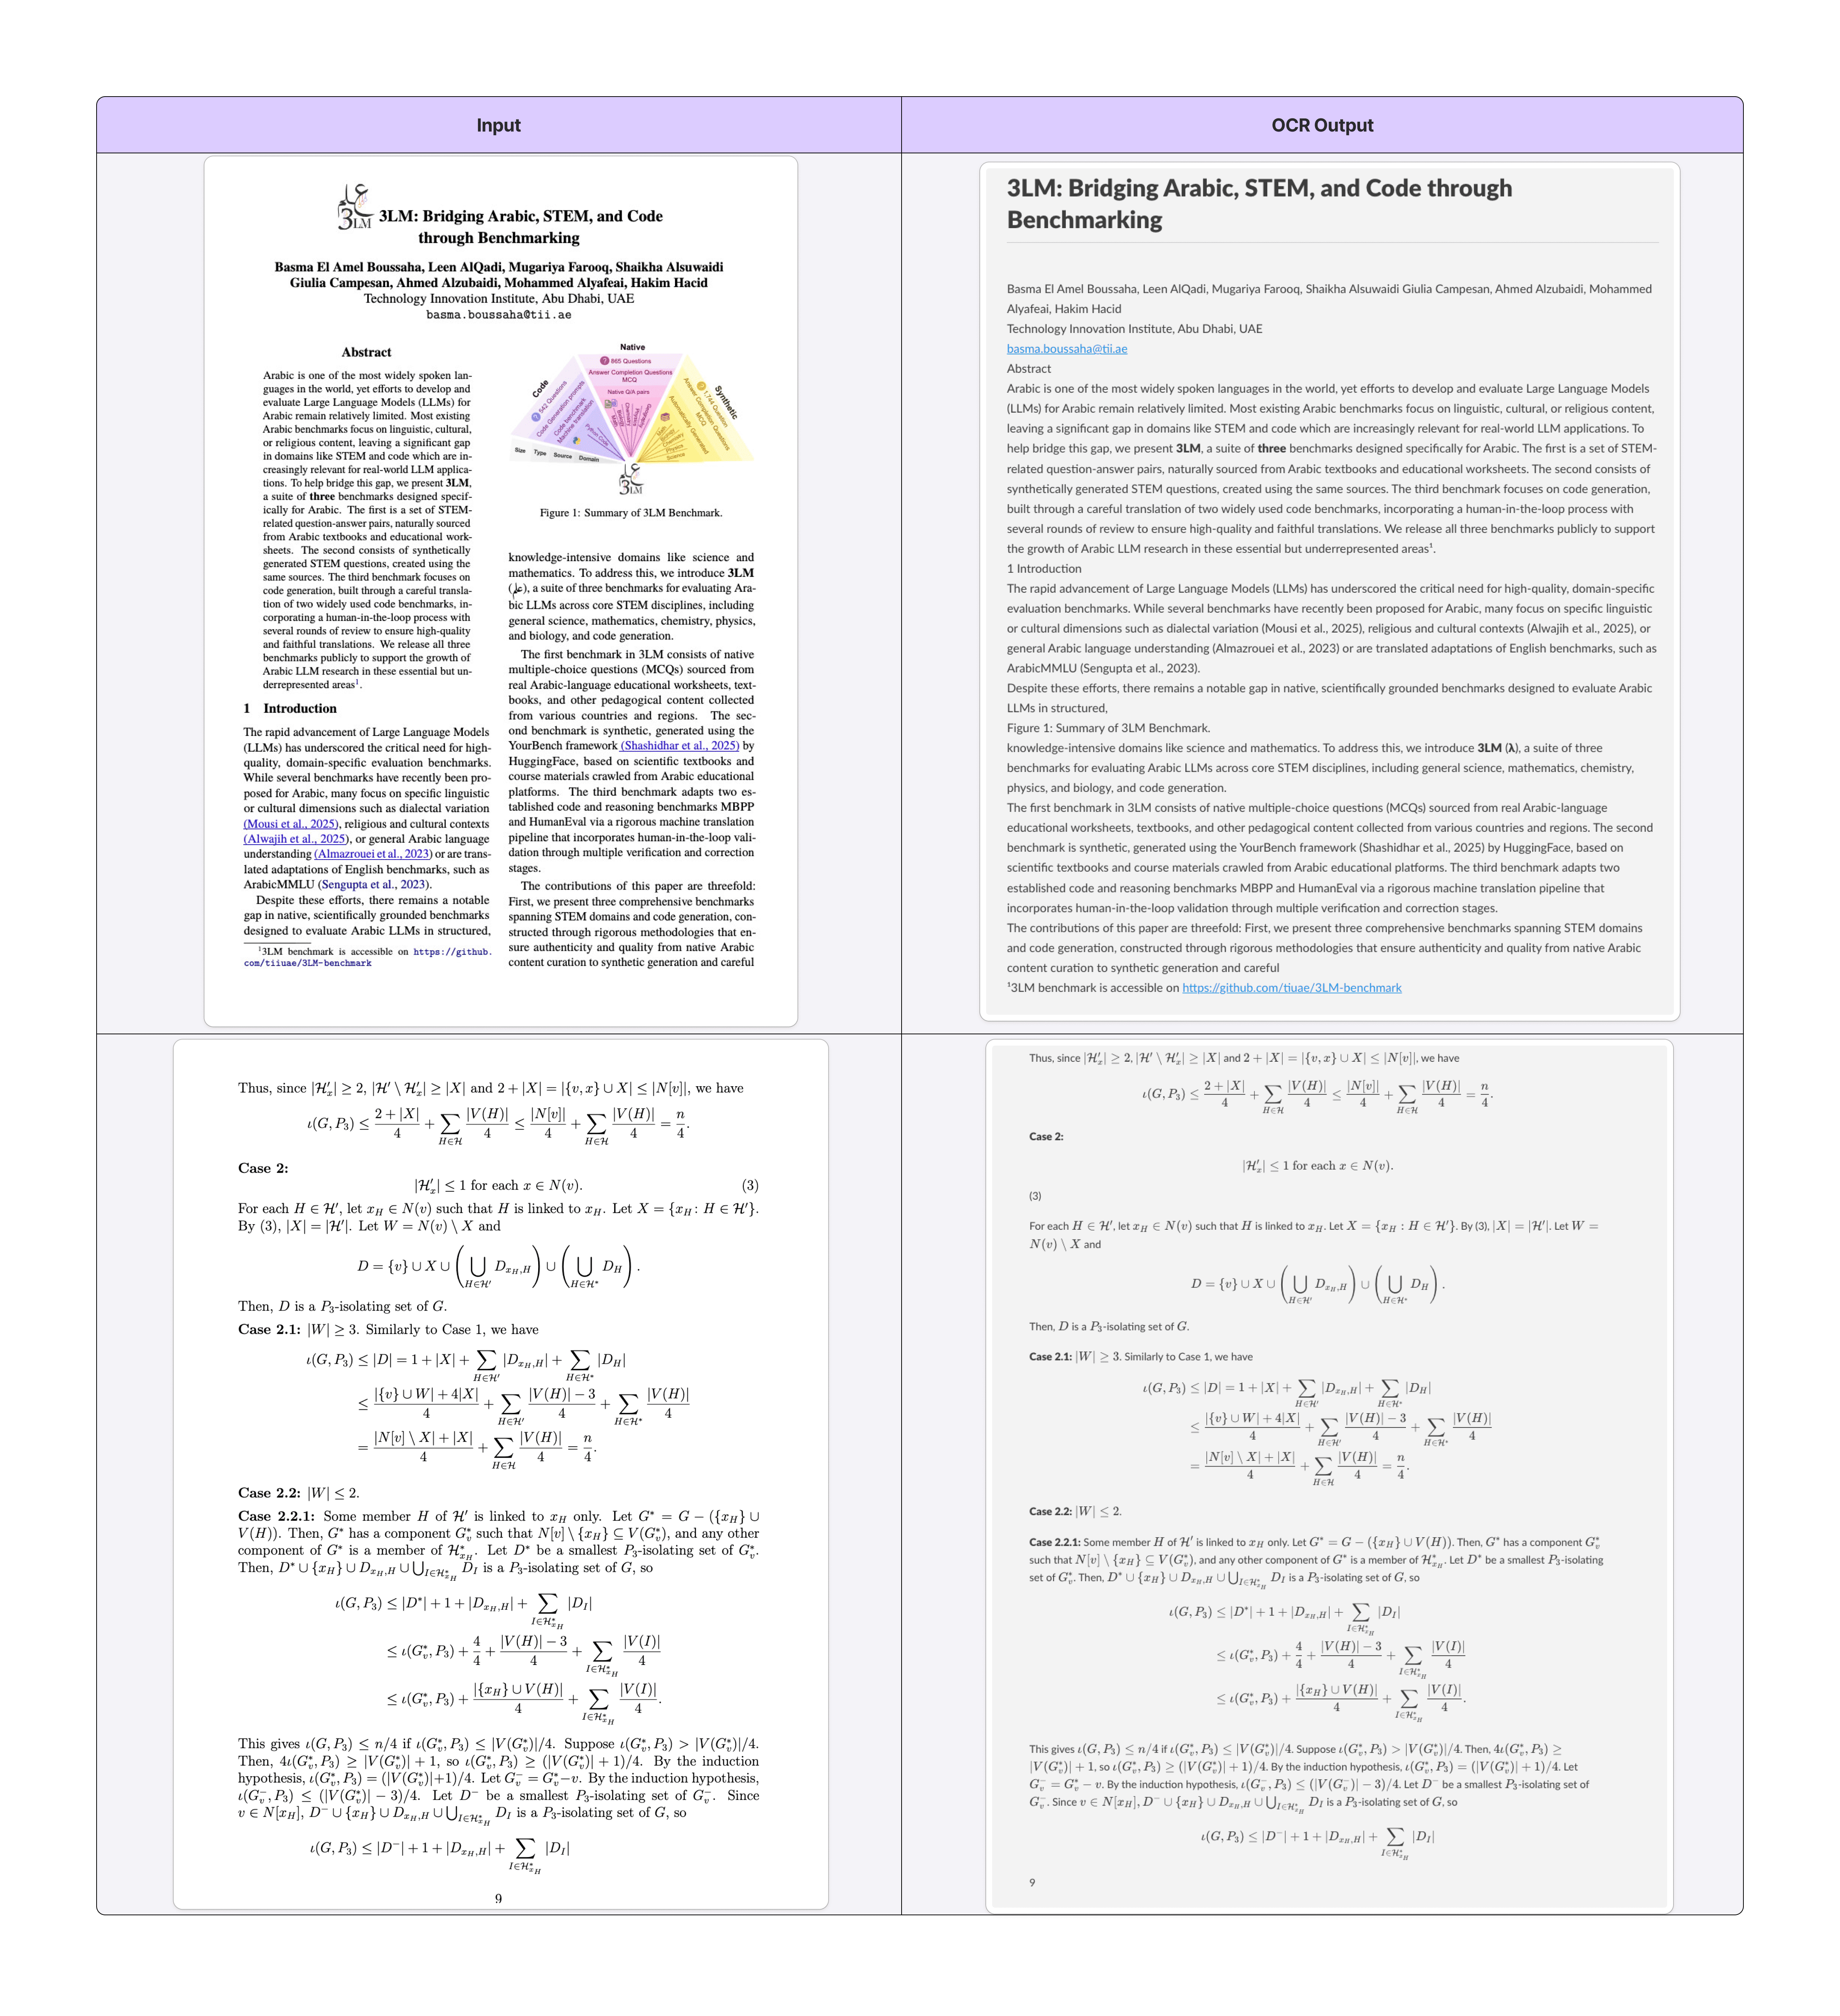
\includegraphics[width=1.0\textwidth, trim=4.5cm 4.5cm 4.5cm 4.5cm, clip]{figures/appendix_ocr/scientific.png}
  \caption{FalconOCR outputs for samples with arxiv papers, scientific formulae. Best viewed zoomed-in.}
  \label{fig:paper2_ocr}
\end{figure}


\begin{figure}[thb]
  \centering
  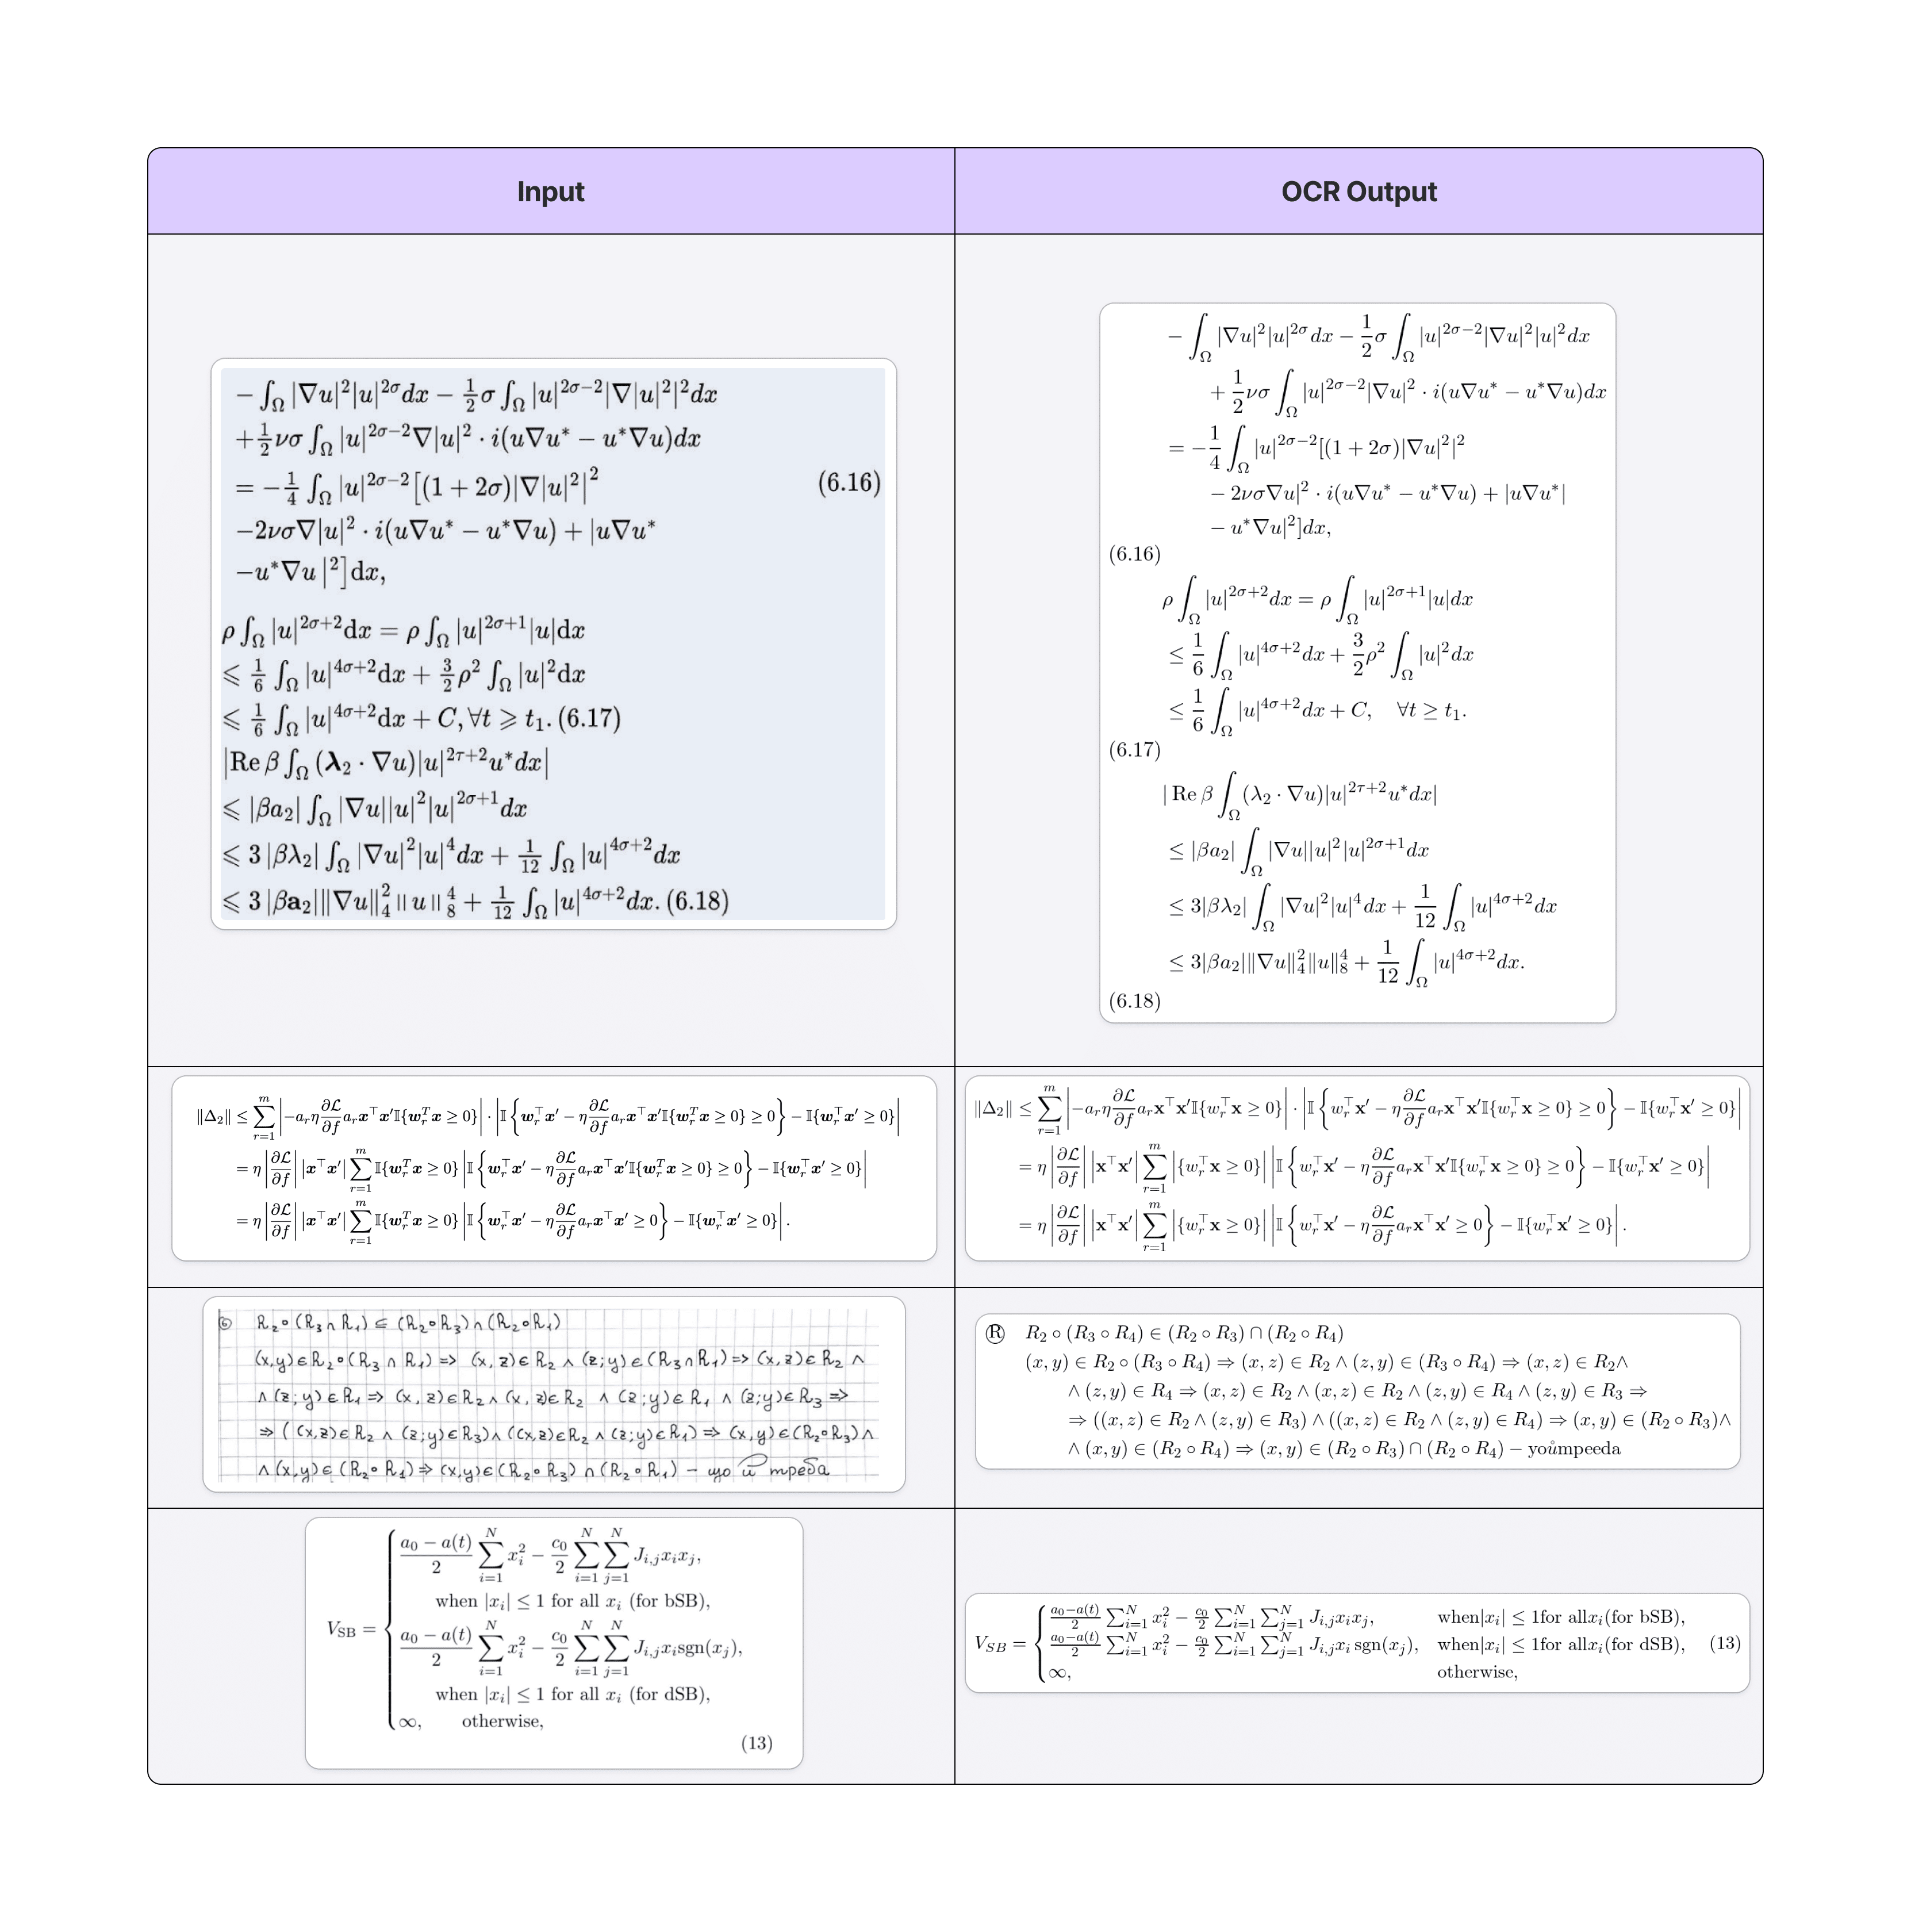
\includegraphics[width=1.0\textwidth, trim=4.5cm 4.5cm 4.5cm 4.5cm, clip]{figures/appendix_ocr/formulas.png}
  \caption{Example outputs for inputs with variations in structure of equations. Best viewed zoomed-in.}
  \label{fig:formulas}
\end{figure}


\begin{figure}[thb]
  \centering
  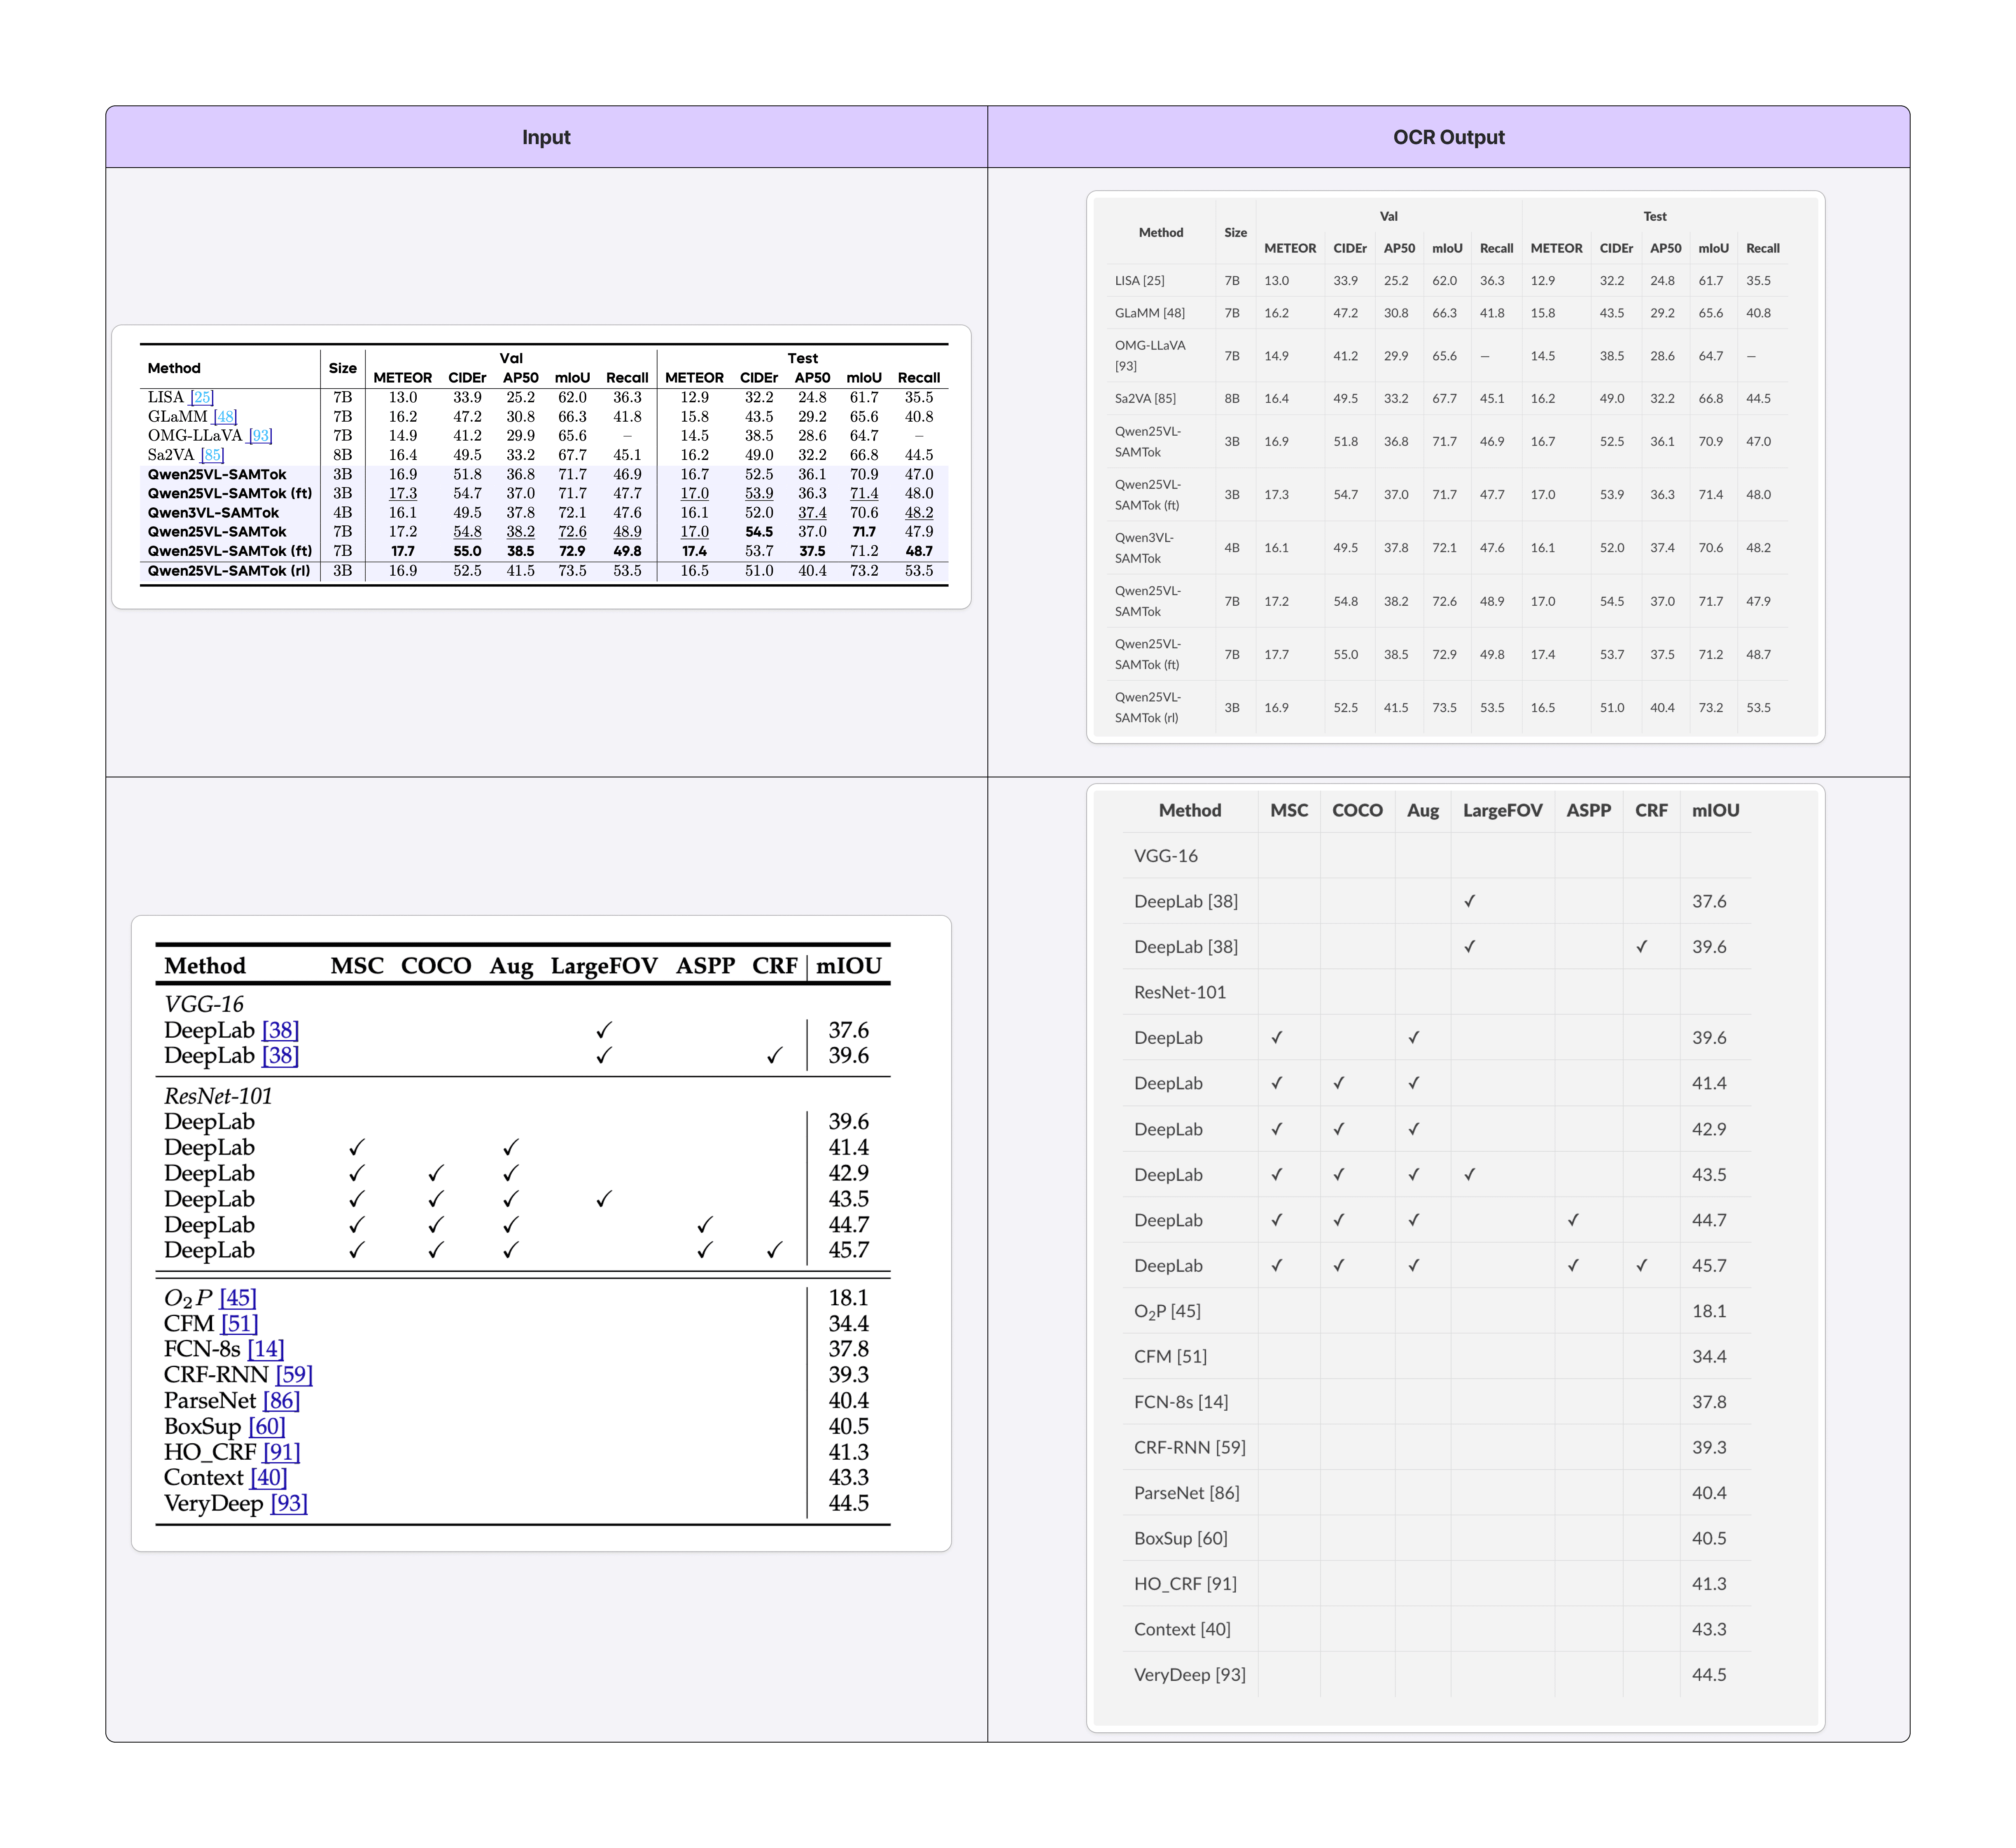
\includegraphics[width=1.0\textwidth, trim=4.5cm 4.5cm 4.5cm 4.5cm, clip]{figures/appendix_ocr/tables.png}
  \caption{Example outputs for inputs with variations in structure of tables - sparse and dense with multi-column headers. Best viewed zoomed-in.}
  \label{fig:tables}
\end{figure}
